\documentclass[a4paper,12pt,oneside]{book}
\usepackage[T1]{fontenc}
\usepackage{multirow}
\usepackage{mathrsfs}
\usepackage{lscape}
\usepackage{amsmath}
\usepackage{amssymb}
\usepackage{xspace}
\usepackage{algorithm}
\usepackage{algorithmic}
\usepackage{cmap}
\usepackage{lmodern}
\usepackage{longtable}
\usepackage{pifont}
\usepackage{microtype}
\usepackage[french]{babel}
\usepackage{acronym}
\usepackage{placeins}
\usepackage{url}
\usepackage{siunitx}
\usepackage[french]{isodate}
\usepackage[figuresright]{rotating}
\usepackage{alltt}
\usepackage{fancyvrb}
\usepackage{listings}
\usepackage{graphicx}
\usepackage{array}
\usepackage{tabularx}
\usepackage{longtable}
\usepackage{booktabs}
\usepackage{multirow}
\usepackage[bottom]{footmisc}
\usepackage[numbers,sectionbib]{natbib}
\usepackage{float}
\usepackage{tabularx}
\usepackage{array}
\usepackage{placeins}
\usepackage[
  hyperfootnotes=true,
  plainpages=false,
  pdfpagelabels=true
]{hyperref}
\usepackage{pgfgantt}
\usepackage{tikz}
\usepackage{makeidx}
\usepackage{multicol}
\usepackage[french]{minitoc}
\usepackage{bookmark}
\usepackage{longtable}
\usepackage{xltabular}
\hypersetup{
  bookmarksnumbered=true,
  breaklinks=true,
  colorlinks=true,
  linkcolor=blue,
  urlcolor=blue,
  citecolor=blue,
}

\makeatletter
\renewcommand{\fnum@figure}{\small\textbf{\figurename~\thefigure}}
\makeatother

\usepackage{vmargin}
\setmarginsrb{3cm}{2.5cm}{2.5cm}{2.5cm}{0cm}{1.5cm}{0cm}{1cm}
\setlength{\skip\footins}{1cm}

\selectlanguage{french}
\renewcommand{\baselinestretch}{1.3}
\renewcommand{\labelitemi}{\large $\bullet$}
\renewcommand{\labelitemii}{\large $\circ$}

\begin{document}

\graphicspath{{images/}}
\setcounter{secnumdepth}{4}
\setcounter{tocdepth}{3}
\setcounter{NAT@ctr}{0}
\setcounter{mtc}{6}

\frontmatter
\dominitoc

%% Sommaire / Table des matières
\tableofcontents
\listoffigures
\listoftables

\mainmatter

%% ============================================================
%%  Introduction Générale
%% ============================================================
 
%% ============================================================
%%  General Introduction
%% ============================================================
\chapter*{General Introduction}
\addcontentsline{toc}{chapter}{General Introduction}

Since the dawn of civilization, knowledge transmission has been one of the fundamental
pillars of human progress. In today's digital era, educational systems are facing new
challenges, including the globalization of skills, the diversification of learner profiles,
the rapid evolution of technology, and the growing demand for accessible and flexible
learning opportunities. In this context, e-learning has emerged as an effective solution,
providing learners with personalized, flexible, and accessible educational experiences.

In Tunisia and across the MENA region, the education and training sector is undergoing a
significant digital transformation. Universities, training centers, educational institutions,
and independent instructors are increasingly seeking digital solutions capable of managing
their educational activities while preserving their organizational structures and teaching
methodologies. This growing demand highlights the need for a multi-organizational platform
that enables multiple institutions to operate within a shared infrastructure while maintaining
their autonomy, security, and customization requirements.

It is within this context that the present final-year project was carried out at
\textbf{YohaTech Monastir} under the title:

\begin{center}
\textit{``Development and Implementation of an AI-Powered Multi-Organization Learning Management System''}
\end{center}
Tesla Academy is a Learning Management System (LMS) designed around a multi-organization architecture. The platform enables multiple organizations, such as universities, training centers, educational institutions, and independent instructors, to manage their educational activities through isolated and secure workspaces while sharing a common technological infrastructure.

In addition to traditional LMS functionalities, Tesla Academy incorporates Artificial
Intelligence technologies aimed at enhancing both teaching and learning experiences. The
platform provides intelligent educational assistance, automated question generation,
assignment evaluation and feedback, content retrieval through Retrieval-Augmented Generation
(RAG), and AI-powered support tools that facilitate knowledge acquisition and improve learner
engagement.

The project was developed using a modern software architecture composed of a web-based
frontend application, a backend service responsible for business logic and data management,
and a dedicated AI microservice that delivers advanced intelligent functionalities. This
architecture ensures modularity, maintainability, scalability, and seamless integration of
AI capabilities within the learning environment.

The primary objective of this project is to design, develop, and deploy a secure, scalable,
and intelligent learning platform capable of serving multiple organizations while leveraging
Artificial Intelligence to improve educational effectiveness, learner support, and overall
user experience.

Finally, this report presents the different phases of the project, from the study of the
existing solutions and requirements analysis to system design, implementation, testing, and
deployment. It concludes with a summary of the achievements and proposes future enhancements
for the continuous evolution of Tesla Academy.
 


%% ============================================================
%%  Chapitre 1 — Cadre du projet 
%% ========================================================


%% ============================================================
%%  Chapter 6 — Release 3: Advanced Services and AI Features
%% ============================================================
\begingroup
\renewcommand{\baselinestretch}{0.85}
\chapter{Release 3: Advanced Services and AI Features}
\minitoc
\endgroup
\newpage

%% ------------------------------------------------------------
\section*{Introduction}
\addcontentsline{toc}{section}{Introduction}
%% ------------------------------------------------------------

This chapter presents the implementation of the third and final release of Tesla Academy.
Release 3 corresponds to Sprints 5 and 6 and introduces the advanced services that
differentiate the platform from conventional LMS solutions: online payment processing,
live session management, and a comprehensive suite of AI-powered educational features.

Sprint 5 covers paid course purchases, payment verification, payment history, and live
session scheduling, start, and participation. Sprint 6 introduces the contextual AI
learning assistant, AI-assisted assignment feedback, automatic question generation,
AI-powered visual theme generation, global platform indicators for the Super Administrator,
and the final platform validation and deployment.

%% ------------------------------------------------------------
\section{Sprint Backlog}
%% ------------------------------------------------------------

\begin{table}[H]
\centering
\caption{Sprint Backlog — Release 3}
\label{tab:backlog_r3}
\renewcommand{\arraystretch}{1.25}
\footnotesize
\begin{tabularx}{\textwidth}{|p{1.4cm}|p{1.5cm}|p{2.8cm}|p{6.8cm}|p{1.5cm}|}
\hline
\textbf{Sprint} & \textbf{Code} & \textbf{Feature} & \textbf{User Story} & \textbf{Est. (h)} \\
\hline
\multirow{7}{*}{Sprint 5}
  & US-042 & Buy course & Purchase a paid course from the platform & 24 \\
  \cline{2-5}
  & US-043 & Payment confirmation & Confirm payment and activate course enrollment & 16 \\
  \cline{2-5}
  & US-044 & Payment history & Consult payment history & 8 \\
  \cline{2-5}
  & US-045 & Schedule live session & Schedule a live session with date, time, and duration & 16 \\
  \cline{2-5}
  & US-046 & Start live session & Start a live session using the live session service & 16 \\
  \cline{2-5}
  & US-047 & Join live session & Join a live session from the student workspace & 8 \\
  \cline{2-5}
  & US-048 & Automatic session summary & Generate a summary after a live session & 16 \\
\hline
\multirow{7}{*}{Sprint 6}
  & US-049 & Contextual AI assistant & Ask the AI assistant questions related to course content & 24 \\
  \cline{2-5}
  & US-050 & Assignment feedback with AI & Receive AI-assisted feedback on assignments & 16 \\
  \cline{2-5}
  & US-051 & Question generation & Generate quiz questions automatically & 16 \\
  \cline{2-5}
  & US-052 & AI theme generation & Generate a visual theme from a text description & 16 \\
  \cline{2-5}
  & US-053 & Theme validation & Validate the generated theme before applying it & 8 \\
  \cline{2-5}
  & US-054 & Global indicators & Consult global platform indicators & 16 \\
  \cline{2-5}
  & US-055 & Final validation and deployment & Perform final validation and deploy the platform & 16 \\
\hline
\end{tabularx}
\end{table}

%% ------------------------------------------------------------
\section{Functional and Technical Specifications}
%% ------------------------------------------------------------

\subsection{Payment Processing (US-042, US-043, US-044)}

\begin{table}[H]
\centering
\caption{Specification — Paid Course Purchase}
\label{tab:payment_spec}
\renewcommand{\arraystretch}{1.2}
\begin{tabularx}{\textwidth}{|p{3.5cm}|X|}
\hline
\textbf{User Stories} & US-042, US-043, US-044 — Course purchase, payment confirmation, payment history. \\
\hline
\textbf{Business Rules} &
\begin{itemize}[noitemsep, topsep=2pt]
  \item Paid course enrollment requires a successful payment transaction;
  \item Two payment providers are supported: \textbf{Konnect} and \textbf{Flouci},
        both supporting Tunisian Dinar (TND);
  \item Each organization configures its own payment credentials in its
        \texttt{OrganizationConfig};
  \item Payment amounts are expressed in millimes (1 TND = 1000 millimes);
  \item An \texttt{Order} record is created upon checkout initiation with status
        \texttt{PENDING}, and updated to \texttt{SUCCESS} or \texttt{FAILED} after
        payment gateway callback verification;
  \item Upon confirmed payment, the student is automatically enrolled in the purchased
        course via a \texttt{BatchEnrollment} record.
\end{itemize} \\
\hline
\textbf{Technical Specification} &
\begin{itemize}[noitemsep, topsep=2pt]
  \item Konnect integration uses the \texttt{/payments/init-payment} API endpoint to
        generate a payment URL; verification is performed via the
        \texttt{/payments/:ref} endpoint;
  \item Flouci integration uses a public/private key pair stored per organization;
  \item The payment mode is determined by the \texttt{paymentMode} field in
        \texttt{OrganizationConfig}: \texttt{per\_course} or \texttt{subscription};
  \item Callback URLs include the \texttt{orderId} parameter, allowing the backend to
        match and update the corresponding \texttt{Order} record;
  \item Enrollment is granted by the \texttt{grantOrderEntitlements} function only after
        payment status is confirmed as \texttt{SUCCESS}.
\end{itemize} \\
\hline
\textbf{Acceptance Criteria} &
\begin{itemize}[noitemsep, topsep=2pt]
  \item A student can initiate checkout for a paid course;
  \item After successful payment, the student is enrolled and can access course content;
  \item A failed or cancelled payment does not grant enrollment;
  \item The student can view their payment history from their dashboard.
\end{itemize} \\
\hline
\end{tabularx}
\end{table}

\subsection{Live Session Management (US-045 to US-048)}

\begin{table}[H]
\centering
\caption{Specification — Live Sessions}
\label{tab:livekit_spec}
\renewcommand{\arraystretch}{1.2}
\begin{tabularx}{\textwidth}{|p{3.5cm}|X|}
\hline
\textbf{User Stories} & US-045 to US-048 — Schedule, start, join, and summarize live sessions. \\
\hline
\textbf{Business Rules} &
\begin{itemize}[noitemsep, topsep=2pt]
  \item An instructor schedules a session by providing a title, course association,
        date, time, and expected duration;
  \item Enrolled students receive an email notification when a new session is scheduled;
  \item The instructor starts the session from their workspace, which transitions the
        \texttt{Schedule} status to \texttt{LIVE} and issues a host-role LiveKit token;
  \item Students join using a participant-role token; they can view and hear but cannot
        publish audio/video by default unless the host grants permission;
  \item After the session ends, if transcription data is available, the AI microservice
        automatically generates a structured summary of the session.
\end{itemize} \\
\hline
\textbf{Technical Specification} &
\begin{itemize}[noitemsep, topsep=2pt]
  \item Live sessions use \textbf{LiveKit}, an open-source WebRTC infrastructure;
  \item A \texttt{LiveKit JWT token} is generated server-side using the
        \texttt{LIVEKIT\_API\_KEY} and \texttt{LIVEKIT\_API\_SECRET} environment
        variables;
  \item Host tokens carry \texttt{canPublish: true} and \texttt{canSubscribe: true};
        student tokens carry \texttt{canPublish: false};
  \item Session transcription is collected incrementally on the client and sent to the
        backend after the session ends via the \texttt{transcriptDraft} field;
  \item The AI summarization endpoint (\texttt{POST /internal/v1/schedules/summarize})
        receives the transcript and returns a structured summary stored in the
        \texttt{aiSummary} field of the \texttt{Schedule} record;
  \item A collaborative whiteboard is available per session via the
        \texttt{ScheduleWhiteboard} entity.
\end{itemize} \\
\hline
\textbf{Acceptance Criteria} &
\begin{itemize}[noitemsep, topsep=2pt]
  \item An instructor can schedule and start a session; students can join using the
        provided room token;
  \item Session participants can communicate in real time;
  \item After the session, a summary is automatically generated and displayed;
  \item Completed sessions cannot be restarted.
\end{itemize} \\
\hline
\end{tabularx}
\end{table}

\subsection{Contextual AI Assistant (US-049)}

\begin{table}[H]
\centering
\caption{Specification — Contextual AI Assistant (RAG Chat)}
\label{tab:rag_spec}
\renewcommand{\arraystretch}{1.2}
\begin{tabularx}{\textwidth}{|p{3.5cm}|X|}
\hline
\textbf{User Story} & US-049 — As a student, I want to ask the AI assistant questions about course content so that I can get contextual explanations. \\
\hline
\textbf{Business Rules} &
\begin{itemize}[noitemsep, topsep=2pt]
  \item The AI assistant is scoped to the content of the course the student is
        currently viewing;
  \item Responses are grounded in the indexed course content through RAG;
  \item Each organization uses its own OpenRouter API key for AI calls;
  \item Conversation history is maintained within the session for multi-turn coherence.
\end{itemize} \\
\hline
\textbf{Technical Specification} &
\begin{itemize}[noitemsep, topsep=2pt]
  \item When educational content (YouTube video, PDF, text) is published, the backend
        triggers the \texttt{POST /internal/v1/content/index} endpoint to extract text
        and store vector embeddings in the \texttt{content\_embeddings} pgvector table;
  \item When the student sends a message, the AI microservice computes a query
        embedding, retrieves the top-$k$ most similar content chunks via cosine
        similarity, and injects them into the system prompt;
  \item The language model call is made through OpenRouter using the configured model
        (default: \texttt{google/gemini-flash-1.5});
  \item The response includes metadata: \texttt{ragChunksUsed} and \texttt{ragStatus},
        allowing the frontend to indicate whether retrieval was successful.
\end{itemize} \\
\hline
\textbf{Acceptance Criteria} &
\begin{itemize}[noitemsep, topsep=2pt]
  \item A student can ask a question and receive a contextually relevant answer;
  \item The assistant references information from the indexed course content;
  \item The conversation history is maintained within the session.
\end{itemize} \\
\hline
\end{tabularx}
\end{table}

\subsection{AI-Assisted Assignment Feedback (US-050)}

\begin{table}[H]
\centering
\caption{Specification — AI Assignment Feedback}
\label{tab:ai_feedback_spec}
\renewcommand{\arraystretch}{1.2}
\begin{tabularx}{\textwidth}{|p{3.5cm}|X|}
\hline
\textbf{User Story} & US-050 — As a student, I want to receive automatic AI-assisted feedback on my assignment so that I can understand my mistakes. \\
\hline
\textbf{Business Rules} &
\begin{itemize}[noitemsep, topsep=2pt]
  \item AI feedback is generated automatically when a student submits an assignment;
  \item The feedback analyzes each question response against the correct answer and
        the defined evaluation criteria;
  \item AI feedback is stored alongside the submission and displayed to the student;
  \item AI feedback does not replace the instructor's grade; it is supplementary.
\end{itemize} \\
\hline
\textbf{Technical Specification} &
\begin{itemize}[noitemsep, topsep=2pt]
  \item Upon submission, the backend compiles a structured prompt containing the
        assignment questions, the student's answers, and the correct answers;
  \item The prompt is sent to \texttt{POST /internal/v1/assignments/feedback};
  \item The AI response is expected as structured JSON containing per-question feedback
        and an overall assessment;
  \item The result is stored in the \texttt{AssignmentAiFeedback} table and linked
        to the submission;
  \item Weak concept flags are extracted from the feedback and stored in
        \texttt{WeakConceptFlag} for long-term student progress analysis.
\end{itemize} \\
\hline
\textbf{Acceptance Criteria} &
\begin{itemize}[noitemsep, topsep=2pt]
  \item After submitting an assignment, the student sees an AI-generated feedback
        section alongside their submission;
  \item The feedback addresses each question individually;
  \item The feedback is generated asynchronously and does not block the submission flow.
\end{itemize} \\
\hline
\end{tabularx}
\end{table}

\subsection{AI Question Generation (US-051)}

\begin{table}[H]
\centering
\caption{Specification — AI Question Generation}
\label{tab:qgen_spec}
\renewcommand{\arraystretch}{1.2}
\begin{tabularx}{\textwidth}{|p{3.5cm}|X|}
\hline
\textbf{User Story} & US-051 — As an instructor, I want to generate quiz questions automatically so that I can save time when preparing assessments. \\
\hline
\textbf{Business Rules} &
\begin{itemize}[noitemsep, topsep=2pt]
  \item The instructor specifies a topic, difficulty level, number of questions, and
        question type;
  \item The platform generates the questions using the LLM and presents them for review
        before insertion into the assignment;
  \item The instructor can edit, discard, or accept individual generated questions.
\end{itemize} \\
\hline
\textbf{Technical Specification} &
\begin{itemize}[noitemsep, topsep=2pt]
  \item A structured prompt is sent to
        \texttt{POST /internal/v1/assignments/generate-questions};
  \item The response is expected as JSON matching the internal
        \texttt{AssignmentQuestion} schema;
  \item A validation layer (\texttt{validateGeneratedAssignmentQuestion}) ensures that
        generated questions conform to the schema before they are offered to the instructor.
\end{itemize} \\
\hline
\textbf{Acceptance Criteria} &
\begin{itemize}[noitemsep, topsep=2pt]
  \item The instructor can request question generation by filling a short form;
  \item The generated questions appear in the assignment editor for review;
  \item The instructor can selectively add generated questions to the assignment.
\end{itemize} \\
\hline
\end{tabularx}
\end{table}

\subsection{AI Visual Theme Generation (US-052, US-053)}

\begin{table}[H]
\centering
\caption{Specification — AI Theme Generation}
\label{tab:theme_spec}
\renewcommand{\arraystretch}{1.2}
\begin{tabularx}{\textwidth}{|p{3.5cm}|X|}
\hline
\textbf{User Stories} & US-052, US-053 — Generate and validate an AI-powered visual theme. \\
\hline
\textbf{Business Rules} &
\begin{itemize}[noitemsep, topsep=2pt]
  \item The Organization Administrator provides a textual brand description as input;
  \item The AI microservice generates a complete CSS variable theme for the organization;
  \item The administrator previews the generated theme before applying it;
  \item Applying the theme updates the \texttt{customCss} field in \texttt{OrganizationConfig},
        which is injected dynamically into the student-facing frontend.
\end{itemize} \\
\hline
\textbf{Technical Specification} &
\begin{itemize}[noitemsep, topsep=2pt]
  \item The \texttt{generate\_theme\_bundle} function in \texttt{theme\_engine.py}
        constructs a prompt and calls OpenRouter to obtain a JSON payload containing
        \texttt{primaryColor}, \texttt{secondaryColor}, \texttt{fontFamily}, and
        \texttt{customCss};
  \item Generated CSS is expressed entirely in \texttt{oklch()} color format to ensure
        consistency with the Tailwind CSS v4 design token system;
  \item A \texttt{\_sanitize\_css} function validates the output against forbidden
        patterns (external URLs, \texttt{@import}, \texttt{expression()}), then merges
        the AI output with a deterministic scaffold to guarantee all required CSS
        variables are present;
  \item The final theme includes both \texttt{:root} (light mode) and \texttt{.dark}
        (dark mode) variable blocks;
  \item All 51 required CSS variables defined in \texttt{REQUIRED\_THEME\_VARS} must
        be present in the sanitized output; missing variables are filled from the
        scaffold.
\end{itemize} \\
\hline
\textbf{Acceptance Criteria} &
\begin{itemize}[noitemsep, topsep=2pt]
  \item The administrator enters a brand description and receives a generated theme;
  \item A live preview shows the theme applied to a sample of the platform UI;
  \item Clicking apply updates the organization's visual appearance across the platform;
  \item Invalid or unsafe CSS is never applied.
\end{itemize} \\
\hline
\end{tabularx}
\end{table}

%% ------------------------------------------------------------
\section{Design}
%% ------------------------------------------------------------

\subsection{Static Modeling}

\subsubsection{Class Diagram}

Figure~\ref{fig:class_r3} presents the class diagram for Release 3, focusing on the
payment, live session, and AI feature entities.

\begin{figure}[H]
  \centerline{\includegraphics[width=\textwidth]{class_diagram_r3.png}}
  \caption{Class Diagram — Release 3}
  \label{fig:class_r3}
\end{figure}

The main entities and relationships introduced in this release are:

\begin{itemize}
  \item An \texttt{Order} links a \texttt{User} to a purchased entity (a \texttt{Batch}
        or \texttt{TestSeries}) and tracks the payment status and provider;
  \item A \texttt{Schedule} (live session) belongs to an \texttt{Organization} and is
        optionally associated with a \texttt{Batch}; it tracks the LiveKit room name,
        session status, and transcript;
  \item A \texttt{ScheduleWhiteboard} is a collaborative drawing board associated with
        one \texttt{Schedule};
  \item An \texttt{AssignmentAiFeedback} record stores the AI-generated feedback for
        one \texttt{AssignmentSubmission};
  \item A \texttt{WeakConceptFlag} captures topics identified as weak for a student,
        derived from AI feedback analysis;
  \item The \texttt{OrganizationConfig} entity stores the \texttt{customCss} field
        used to inject the AI-generated theme, as well as payment credentials and
        the OpenRouter API key.
\end{itemize}

\subsection{Dynamic Modeling}

\subsubsection{Payment Flow Sequence Diagram}

Figure~\ref{fig:seq_payment} illustrates the paid course purchase flow. The student
initiates checkout from the course detail page. The backend creates an \texttt{Order}
with status \texttt{PENDING} and calls the payment gateway API to obtain a payment URL.
The student is redirected to the gateway's hosted checkout page. After payment, the
gateway redirects the student to the platform's callback URL. The backend verifies the
payment status via the gateway API and, on success, transitions the order to
\texttt{SUCCESS} and grants the course enrollment.

\begin{figure}[H]
  \centerline{\includegraphics[width=0.95\textwidth]{seq_payment.png}}
  \caption{Paid Course Purchase Sequence Diagram}
  \label{fig:seq_payment}
\end{figure}

\subsubsection{Live Session Sequence Diagram}

Figure~\ref{fig:seq_live} illustrates the live session workflow. The instructor schedules
a session, which triggers enrollment email notifications. At session time, the instructor
clicks \textit{Start}. The backend generates a host-role LiveKit token and updates the
session status to \texttt{LIVE}. Students request a participant token and connect to the
same LiveKit room. After the session ends, the transcript is submitted and the AI
microservice generates a summary.

\begin{figure}[H]
  \centerline{\includegraphics[width=0.95\textwidth]{seq_live_session.png}}
  \caption{Live Session Sequence Diagram}
  \label{fig:seq_live}
\end{figure}

\subsubsection{RAG Chat Sequence Diagram}

Figure~\ref{fig:seq_rag} illustrates the Retrieval-Augmented Generation (RAG) pipeline
used by the contextual AI assistant. When a student sends a message, the AI microservice
generates a vector embedding of the query, searches the \texttt{content\_embeddings}
table for the most semantically similar content chunks, injects these chunks into the
system prompt, and calls the language model via OpenRouter to produce a grounded response.

\begin{figure}[H]
  \centerline{\includegraphics[width=0.9\textwidth]{seq_rag_chat.png}}
  \caption{RAG Chat Sequence Diagram}
  \label{fig:seq_rag}
\end{figure}

\subsubsection{AI Theme Generation Sequence Diagram}

Figure~\ref{fig:seq_theme} illustrates the AI theme generation flow. The administrator
submits a brand description through the theme editor. The backend forwards the request to
the AI microservice, which constructs a structured prompt, calls OpenRouter, parses and
sanitizes the CSS output, and returns the theme bundle. The administrator previews the
result and optionally applies it, which stores the \texttt{customCss} in the organization
configuration and applies it immediately to the student-facing interface.

\begin{figure}[H]
  \centerline{\includegraphics[width=0.9\textwidth]{seq_theme_generation.png}}
  \caption{AI Theme Generation Sequence Diagram}
  \label{fig:seq_theme}
\end{figure}

%% ------------------------------------------------------------
\section{Implementation}
%% ------------------------------------------------------------

\subsection{Payment Integration}

Tesla Academy integrates two Tunisian payment gateways: \textbf{Konnect} and
\textbf{Flouci}. Both gateways operate with TND-denominated transactions expressed in
millimes. The active gateway for each organization is determined by the
\texttt{paymentMode} field in its configuration.

The checkout flow creates a pending \texttt{Order} record, calls the selected gateway
API to generate a hosted payment URL, and redirects the student. The callback handler
verifies the payment reference with the gateway and, on confirmed success, calls
\texttt{grantOrderEntitlements} to create the enrollment. The student is then redirected
to the newly accessible course.

\begin{figure}[H]
  \centerline{\includegraphics[width=\textwidth]{screenshot_checkout.png}}
  \caption{Course Checkout Page — Student View}
  \label{fig:sc_checkout}
\end{figure}

\begin{figure}[H]
  \centerline{\includegraphics[width=\textwidth]{screenshot_payment_history.png}}
  \caption{Payment History — Student Dashboard}
  \label{fig:sc_payment_history}
\end{figure}

\subsection{Live Session Room}

The live session room is built on top of the LiveKit SDK. The instructor's view provides
controls for microphone, camera, screen sharing, and participant management. The student
view provides a viewer layout with audio/video reception and a real-time chat panel. A
collaborative whiteboard panel is also accessible during the session.

Transcription is collected progressively on the client by concatenating speech recognition
segments. After the host ends the session, the accumulated transcript is submitted to the
backend and forwarded to the AI microservice for summary generation. The resulting summary
is stored and displayed to both the instructor and enrolled students.

\begin{figure}[H]
  \centerline{\includegraphics[width=\textwidth]{screenshot_live_session.png}}
  \caption{Live Session Room — Instructor View}
  \label{fig:sc_live_session}
\end{figure}

\begin{figure}[H]
  \centerline{\includegraphics[width=\textwidth]{screenshot_session_summary.png}}
  \caption{AI-Generated Session Summary}
  \label{fig:sc_session_summary}
\end{figure}

\subsection{Contextual AI Learning Assistant}

The AI assistant is accessible to students from within any course page as a side panel.
The student types a question in natural language; the assistant retrieves relevant content
chunks from the course materials using vector similarity search and constructs a
contextually grounded response.

The content indexing pipeline is triggered automatically when an instructor publishes
a content item. For YouTube videos, the transcript is extracted using the YouTube
Transcript API. For PDF documents, text is extracted with \texttt{pypdf}. The extracted
text is chunked and stored as vector embeddings in the \texttt{content\_embeddings} table
via the \texttt{pgvector} extension.

\begin{figure}[H]
  \centerline{\includegraphics[width=\textwidth]{screenshot_ai_assistant.png}}
  \caption{Contextual AI Learning Assistant — Student View}
  \label{fig:sc_ai_assistant}
\end{figure}

\subsection{AI-Assisted Assignment Feedback and Question Generation}

When a student submits an assignment, the backend triggers an asynchronous AI feedback
request. The feedback analyzes each response against the expected answer and the assignment
grading criteria. The result is displayed to the student in a structured panel alongside
their submission.

The question generation interface allows instructors to specify a topic, question type,
difficulty, and desired count. The AI returns a set of structured questions that the
instructor can review, edit, and add to an assignment with a single click.

\begin{figure}[H]
  \centerline{\includegraphics[width=\textwidth]{screenshot_ai_feedback.png}}
  \caption{AI Assignment Feedback Panel — Student View}
  \label{fig:sc_ai_feedback}
\end{figure}

\begin{figure}[H]
  \centerline{\includegraphics[width=\textwidth]{screenshot_question_gen.png}}
  \caption{AI Question Generation — Instructor View}
  \label{fig:sc_question_gen}
\end{figure}

\subsection{AI Visual Theme Generation}

The theme generator allows the Organization Administrator to describe their brand
identity in free text. The AI microservice constructs a deterministic CSS token scaffold
based on the extracted color keywords and font preferences, then asks the language model
to refine it. The resulting theme defines all 51 required CSS variables in
\texttt{oklch()} color space for both light and dark modes.

The generated CSS is validated to reject any forbidden patterns (external URLs,
executable JavaScript, Tailwind at-rules), merged with the scaffold to ensure
completeness, and returned to the frontend for preview. Upon administrator approval, the
theme is saved in the organization configuration and injected into the platform via a
\texttt{<style>} tag in the HTML head.

\begin{figure}[H]
  \centerline{\includegraphics[width=\textwidth]{screenshot_theme_editor.png}}
  \caption{AI Theme Generation — Organization Administrator View}
  \label{fig:sc_theme_editor}
\end{figure}

\subsection{Super Administrator Global Dashboard}

The Super Administrator dashboard provides a global view of all organizations registered
on the platform. Key indicators displayed include the total number of active organizations,
total registered users across all tenants, total published courses, and platform-wide
revenue. A per-organization breakdown allows the Super Administrator to monitor individual
organization activity and manage activation status.

\begin{figure}[H]
  \centerline{\includegraphics[width=\textwidth]{screenshot_superadmin_dashboard.png}}
  \caption{Global Indicators — Super Administrator Dashboard}
  \label{fig:sc_superadmin_dashboard}
\end{figure}

%% ------------------------------------------------------------
\section*{Conclusion}
\addcontentsline{toc}{section}{Conclusion}
%% ------------------------------------------------------------

This chapter presented the implementation of Release 3 and completed the full description
of the Tesla Academy platform. The third release introduced the advanced services that
define the platform's competitive positioning: Tunisian payment gateway integration with
Konnect and Flouci, real-time live sessions powered by LiveKit with automatic AI
summarization, and a comprehensive AI feature suite including a RAG-based contextual
learning assistant, AI-assisted assignment feedback, automatic question generation, and
AI-powered visual theme generation.

Together, the three releases of Tesla Academy deliver a complete, multi-tenant, and
AI-enhanced Learning Management System adapted to the needs of Tunisian and regional
educational institutions. The platform is designed to be scalable, maintainable, and
extensible, providing a solid foundation for continued development and market deployment.

 

%% ============================================================
%%  Chapitre 2 — Analyse et Spécification des Besoins %% ============================================================
%%  Chapter 2 — Requirements Analysis, Planning and Architecture
%% ============================================================

\chapter{Requirements Analysis, Planning and Architecture}
\minitoc
\newpage

%% ------------------------------------------------------------
\section*{Introduction}
\addcontentsline{toc}{section}{Introduction}
%% ------------------------------------------------------------

This chapter presents the requirements analysis, project planning, and system architecture
of the \textbf{Tesla Academy} platform. It begins by identifying the main actors and their
responsibilities, then describes the functional and non-functional requirements. It
continues with the project planning approach based on Scrum, and concludes with the global
system architecture, the technology stack, and the database design that underpin the
implementation of the platform.

%% ============================================================
\section{Requirements Analysis}
%% ============================================================

Requirements analysis is a fundamental step in any software engineering project. It makes
it possible to clearly define what the system must provide in terms of functionalities and
what quality constraints it must satisfy. In the case of Tesla Academy, this analysis
focuses on the needs of the different user profiles and on the constraints related to
security, performance, scalability, usability, and maintainability.

%% ----------------------------
\subsection{Identification of Actors}
%% ----------------------------

The analysis of the Tesla Academy platform led to the identification of four main actors.
Each actor has specific responsibilities, permissions, and interactions with the system.

\begin{itemize}

  \item \textbf{Super Administrator}: responsible for the global administration of the
        platform. This actor supervises organizations, monitors platform activity, manages
        global indicators, and ensures the proper operation of the system.

  \item \textbf{Organization Administrator}: responsible for the management of a specific
        organization. This actor manages instructors, students, courses, payment settings,
        organization configuration, and the general activity within the organization space.

  \item \textbf{Instructor}: responsible for creating and managing educational content.
        This actor creates courses, organizes lessons and resources, prepares assessments,
        publishes announcements, schedules live sessions, and follows learner progress.

  \item \textbf{Student}: the final user of the platform. This actor accesses courses,
        follows lessons, submits assignments, takes quizzes and tests, joins live sessions,
        interacts with the AI assistant, tracks progress, and obtains certificates when
        success conditions are met.

\end{itemize}

%% ----------------------------
\subsection{Functional Requirements}
%% ----------------------------

Functional requirements describe the main services and actions that the platform must offer
to each actor. In Tesla Academy, these requirements are organized according to the
responsibilities of each user profile.

\subsubsection{Super Administrator Requirements}

The Super Administrator operates at the global platform level and has an overview of all
organizations and system activity.

\begin{itemize}
  \item Manage client organizations by creating, updating, activating, or suspending them;
  \item Consult global platform statistics, including the number of organizations, users,
        courses, and generated revenue;
  \item Monitor the general status of the platform and the services used;
  \item Supervise the global settings required for the proper functioning of the system;
  \item Monitor the general use of AI-related functionalities.
\end{itemize}

\subsubsection{Organization Administrator Requirements}

The Organization Administrator manages the private workspace of an organization. This actor
configures the learning environment, manages users, and supervises educational activities.

\begin{itemize}
  \item Manage instructor and student accounts belonging to the organization;
  \item Create, modify, and organize courses, subjects, chapters, and learning content;
  \item Validate, publish, or reject courses prepared by instructors;
  \item Customize the visual identity and general settings of the organization space;
  \item Consult dashboards to monitor enrollments, learner activity, revenue, and course
        evolution;
  \item Manage categories, prices, course access, and organization-specific parameters;
  \item Configure local payment settings when payment features are enabled;
  \item Configure AI-related settings required for intelligent platform services.
\end{itemize}

\subsubsection{Instructor Requirements}

The Instructor uses the platform to prepare, publish, and monitor educational content.
This role is mainly focused on course creation, assessment preparation, and learner support.

\begin{itemize}
  \item Create and edit courses by defining titles, descriptions, levels, categories, and
        learning objectives;
  \item Structure each course into sections, chapters, and lessons;
  \item Add different types of resources, such as uploaded videos, YouTube videos, PDF
        documents, textual content, and external links;
  \item Prepare quizzes, assignments, and tests using different types of questions;
  \item Review student submissions and consult AI-generated feedback when available;
  \item Schedule and conduct live learning sessions;
  \item Publish announcements for students enrolled in the instructor's courses;
  \item Follow learner progress using dashboards and available statistics;
  \item Generate questions or exercises with the support of AI tools when needed.
\end{itemize}

\subsubsection{Student Requirements}

The Student represents the end user of the platform. This actor accesses learning content,
participates in assessments, and follows progress throughout the learning path.

\begin{itemize}
  \item Browse available courses and enroll in authorized courses;
  \item Purchase paid courses or access free courses;
  \item Watch videos, read PDF documents, and consult resources associated with lessons;
  \item Mark lessons as completed and track course progress;
  \item Take quizzes, tests, and evaluations proposed by instructors;
  \item Submit assignments and consult feedback;
  \item Join live sessions planned by instructors;
  \item Interact with the AI assistant to obtain explanations related to course content;
  \item Consult announcements and take personal notes;
  \item Obtain a certificate after completing a course when the required success conditions
        are met.
\end{itemize}

%% ----------------------------
\subsection{General Use Case Diagram}
%% ----------------------------

\begin{figure}[H]
  \centerline{\includegraphics[width=\textwidth]{use_case_general.png}}
  \caption{General Use Case Diagram of Tesla Academy}
  \label{fig:use_case_general}
\end{figure}

The general use case diagram summarizes the main interactions between the four actors and
the Tesla Academy platform. It highlights the major functionalities related to platform
administration, organization management, course creation, learning activities, assessments,
payments, live sessions, certificates, and AI-powered assistance.

%% ----------------------------
\subsection{Non-Functional Requirements}
%% ----------------------------

Non-functional requirements define the expected qualities of the platform independently of
its specific functionalities. They are essential for ensuring that the system remains
secure, reliable, usable, scalable, and maintainable.

\begin{itemize}

  \item \textbf{Security}: the platform must protect user accounts, organization data,
        educational content, and payment-related information. Each user must access only
        the functionalities authorized by their role.

  \item \textbf{Data confidentiality}: the information of one organization must not be
        accessible to other organizations. Courses, students, payments, and statistics must
        remain isolated within each organization space.

  \item \textbf{Performance}: the main pages of the platform must load quickly in order to
        provide smooth navigation. Access to videos, documents, dashboards, and learning
        activities must remain comfortable as the number of users increases.

  \item \textbf{Availability}: the platform must remain accessible during learning periods,
        payment operations, assessments, and live sessions.

  \item \textbf{Usability}: the interface must be clear and easy to use for different user
        profiles, including administrators, instructors, and students. The main actions
        should be simple to find and perform.

  \item \textbf{Compatibility}: the application must work correctly on modern web browsers
        and adapt to different devices, including computers, tablets, and smartphones.

  \item \textbf{Maintainability}: the solution must be organized in a way that facilitates
        bug fixing, future improvements, and the addition of new features without disrupting
        existing functionalities.

  \item \textbf{Scalability}: the platform must be able to support the growth of the number
        of organizations, users, courses, resources, and AI-related requests.

  \item \textbf{Reliability of AI services}: AI-powered functionalities must provide useful
        and coherent responses while remaining aligned with the educational context of the
        platform.

\end{itemize}

%% ============================================================
\section{Project Planning with Scrum}
%% ============================================================

To organize the development of Tesla Academy, an agile approach based on Scrum was adopted.
This methodology makes it possible to divide the project into short iterations called
sprints, allowing the gradual delivery of the main functionalities of the platform. Scrum
also facilitates adaptation to feedback and improves visibility over the progress of the
project.

%% ----------------------------
\subsection{Definition of Scrum Roles}
%% ----------------------------

\begin{figure}[H]
  \centerline{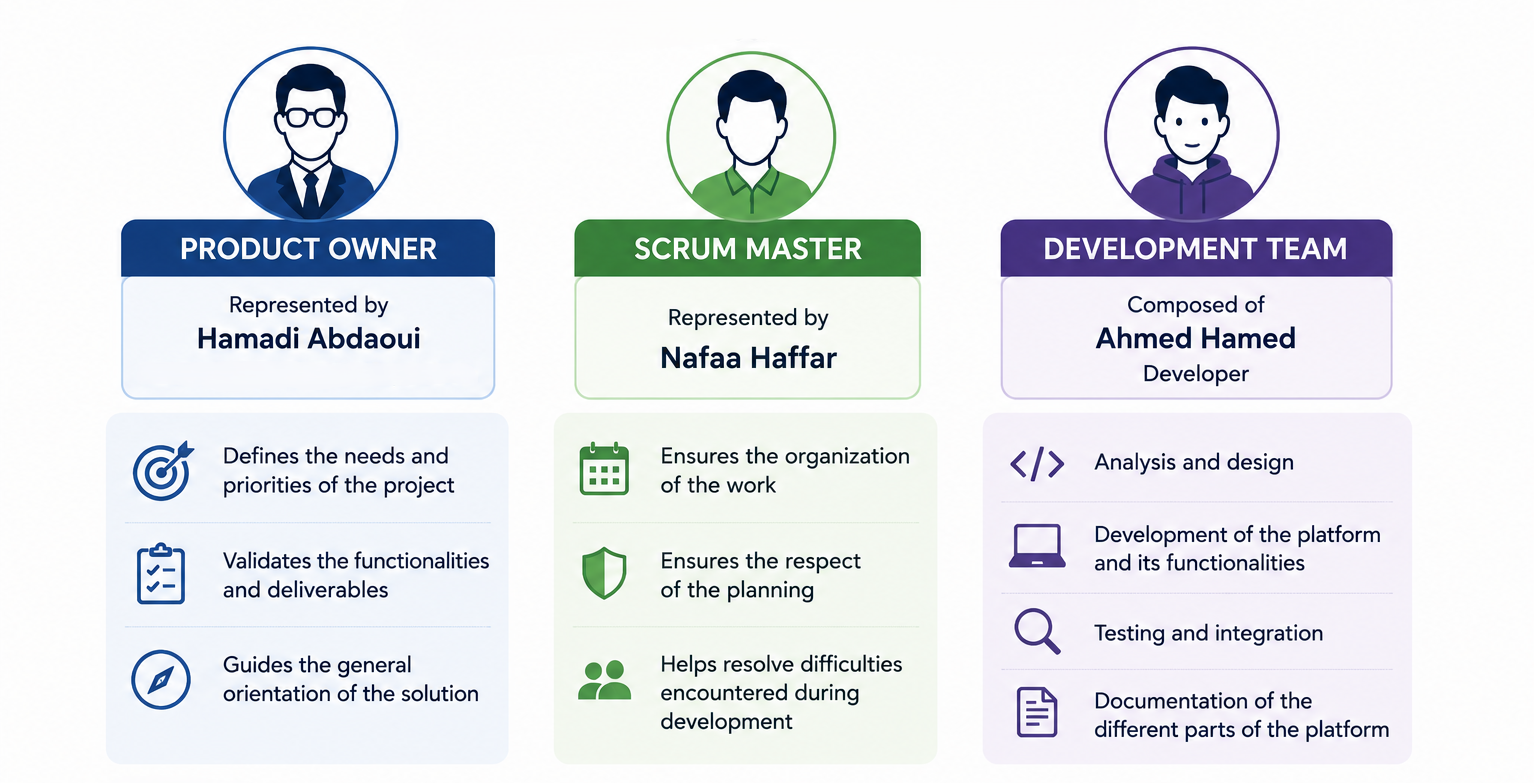
\includegraphics[scale=0.42]{scrum_team_roles.png}}
  \caption{Scrum Team Roles}
  \label{fig:scrum_team_roles}
\end{figure}

Within this project, the Scrum roles are assigned as follows:

\begin{itemize}
  \item \textbf{Product Owner}: represented by the academic and professional supervisors.
        This role contributes to defining the needs, validating the functionalities, and
        guiding the general orientation of the solution;

  \item \textbf{Scrum Master}: represented by the student. This role ensures the
        organization of the work, the respect of the planning, and the resolution of
        difficulties encountered during development;

  \item \textbf{Development Team}: composed of the student, who is responsible for the
        analysis, design, development, testing, integration, and documentation of the
        different parts of the platform.
\end{itemize}

%% ----------------------------
\subsection{Product Backlog}
%% ----------------------------

The Product Backlog contains the main functionalities to be developed in Tesla Academy.
The requirements are expressed as User Stories and organized according to the main actors:
Super Administrator, Organization Administrator, Instructor, Student, and System.

\begingroup
\footnotesize
\setlength{\tabcolsep}{4pt}
\renewcommand{\arraystretch}{1.18}
\begin{longtable}{|p{1.3cm}|p{3cm}|p{2.4cm}|p{7.2cm}|p{1.7cm}|}
  \caption{Product Backlog of Tesla Academy}
  \label{tab:backlog} \\
  \hline
  \textbf{Code} & \textbf{Feature} & \textbf{Actor} & \textbf{User Story} & \textbf{Priority} \\
  \hline
  \endfirsthead

  \hline
  \textbf{Code} & \textbf{Feature} & \textbf{Actor} & \textbf{User Story} & \textbf{Priority} \\
  \hline
  \endhead
  \hline
  \endfoot

  \multicolumn{5}{|l|}{\cellcolor{gray!15}\textbf{Sprint 1 -- Authentication and User Management}} \\
  \hline
  US-001 & Registration & Student & Create a student account using an email and password. & Critical \\
  \hline
  US-002 & Login & All & Log in to the platform securely. & Critical \\
  \hline
  US-003 & Logout & All & Log out from the user account. & High \\
  \hline
  US-004 & Forgot password & All & Reset the account password by email. & High \\
  \hline
  US-005 & User profile & All & Update personal information and avatar. & Medium \\
  \hline
  US-006 & Role-based redirection & System & Redirect the user to the appropriate workspace according to their role. & Critical \\
  \hline
  US-007 & Create organization & Super Admin & Create an organization with its main information. & Critical \\
  \hline
  US-008 & Activate / suspend organization & Super Admin & Activate or suspend an organization. & High \\
  \hline
  US-009 & Instructor management & Organization Admin & Add, update, or suspend instructor accounts. & Critical \\
  \hline

  \multicolumn{5}{|l|}{\cellcolor{gray!15}\textbf{Sprint 2 -- Organization and Course Management}} \\
  \hline
  US-010 & Create course & Instructor & Create a course with a title, description, level, and category. & Critical \\
  \hline
  US-011 & Edit course & Instructor & Modify the information of an existing course. & High \\
  \hline
  US-012 & Submit course & Instructor & Submit a course to the organization administrator for validation. & Critical \\
  \hline
  US-013 & Validate course & Organization Admin & Approve or reject a course submitted by an instructor. & Critical \\
  \hline
  US-014 & Manage categories & Organization Admin & Create and manage course categories. & High \\
  \hline
  US-015 & Add chapters & Instructor & Organize a course into sections, chapters, and lessons. & Critical \\
  \hline
  US-016 & Add resources & Instructor & Add learning resources such as videos, PDFs, text content, or external links. & Critical \\
  \hline
  US-017 & Upload files & Instructor & Upload videos and documents to the storage service. & Critical \\
  \hline
  US-018 & Archive course & Instructor & Archive a course without permanently deleting it. & Low \\
  \hline

  \multicolumn{5}{|l|}{\cellcolor{gray!15}\textbf{Sprint 3 -- Assignments and Learning Experience}} \\
  \hline
  US-019 & Assignment creation & Instructor & Create an assignment by defining its title, instructions, deadline, and evaluation criteria. & Critical \\
  \hline
  US-020 & Assignment resources & Instructor & Attach files, documents, or supporting resources to an assignment. & High \\
  \hline
  US-021 & Assignment publication & Instructor & Publish an assignment and make it available to enrolled students. & High \\
  \hline
  US-022 & Assignment submission & Student & Submit an assignment response with text or attached files before the deadline. & Critical \\
  \hline
  US-023 & Assignment review & Instructor & Review student submissions and provide feedback or grades. & High \\
  \hline
  US-024 & My courses & Student & View the list of courses in which the student is enrolled. & Critical \\
  \hline
  US-025 & Access lesson & Student & Access lesson content such as videos, documents, or text. & Critical \\
  \hline
  US-026 & Complete lesson & Student & Mark a lesson as completed. & Critical \\
  \hline
  US-027 & Progress tracking & Student & Track progress percentage in each course. & High \\
  \hline
  US-028 & Consult assignments & Student & View the list of assignments related to the enrolled courses. & High \\
  \hline
  US-029 & Assignment feedback & Student & Consult feedback or grades received for submitted assignments. & High \\
  \hline
  US-030 & Announcements & Student & Consult announcements published by the instructor. & Medium \\
  \hline

  \multicolumn{5}{|l|}{\cellcolor{gray!15}\textbf{Sprint 4 -- Certificates, Dashboards and Course Catalog}} \\
  \hline
  US-031 & Certificate generation & Student & Obtain a certificate after successfully completing a course. & High \\
  \hline
  US-032 & Certificate download & Student & Download the certificate in PDF format. & High \\
  \hline
  US-033 & Student dashboard & Student & View courses, progress, assignments, and certificates. & High \\
  \hline
  US-034 & Instructor dashboard & Instructor & Monitor course statistics, student progress, and assignment submissions. & High \\
  \hline
  US-035 & Publish announcement & Instructor & Publish announcements for enrolled students. & Medium \\
  \hline
  US-036 & Course catalog & Student & View the list of available courses. & Critical \\
  \hline
  US-037 & Course search & Student & Search for a course by keyword. & Critical \\
  \hline
  US-038 & Catalog filters & Student & Filter courses by category, level, or price. & High \\
  \hline
  US-039 & Course details & Student & View detailed information about a course. & Critical \\
  \hline
  US-040 & Reviews and ratings & Student & Rate and comment on a completed course. & Medium \\
  \hline
  US-041 & Free course enrollment & Student & Enroll in a free course without payment. & High \\
  \hline

  \multicolumn{5}{|l|}{\cellcolor{gray!15}\textbf{Sprint 5 -- Payments and Live Sessions}} \\
  \hline
  US-042 & Buy course & Student & Purchase a paid course from the platform. & Critical \\
  \hline
  US-043 & Payment confirmation & System & Confirm payment and activate course enrollment. & Critical \\
  \hline
  US-044 & Payment history & Student & Consult payment history. & High \\
  \hline
  US-045 & Schedule live session & Instructor & Schedule a live session with a date, time, and duration. & High \\
  \hline
  US-046 & Start live session & Instructor & Start a live session using the live session service. & High \\
  \hline
  US-047 & Join live session & Student & Join a live session from the student workspace. & High \\
  \hline
  US-048 & Automatic session summary & System & Generate a summary after a live session when transcription data is available. & Medium \\
  \hline

  \multicolumn{5}{|l|}{\cellcolor{gray!15}\textbf{Sprint 6 -- AI Features and Deployment}} \\
  \hline
  US-049 & Contextual AI assistant & Student & Ask the intelligent assistant questions related to course content. & Critical \\
  \hline
  US-050 & Assignment feedback with AI & Student & Receive automatic AI-assisted feedback on assignments. & High \\
  \hline
  US-051 & Question generation & Instructor & Generate questions or pedagogical exercises automatically. & High \\
  \hline
  US-052 & AI theme generation & Organization Admin & Generate a visual theme from a textual description. & High \\
  \hline
  US-053 & Theme validation & System & Validate the generated theme before applying it to the platform. & Critical \\
  \hline
  US-054 & Global indicators & Super Admin & Consult global indicators of the platform. & High \\
  \hline
  US-055 & Final validation and deployment & System & Perform final validation, prepare the production environment, and deploy the platform. & Critical \\
  \hline

\end{longtable}
\endgroup

%% ----------------------------
\subsection{User Story Mapping}
%% ----------------------------

\begin{figure}[H]
  \centerline{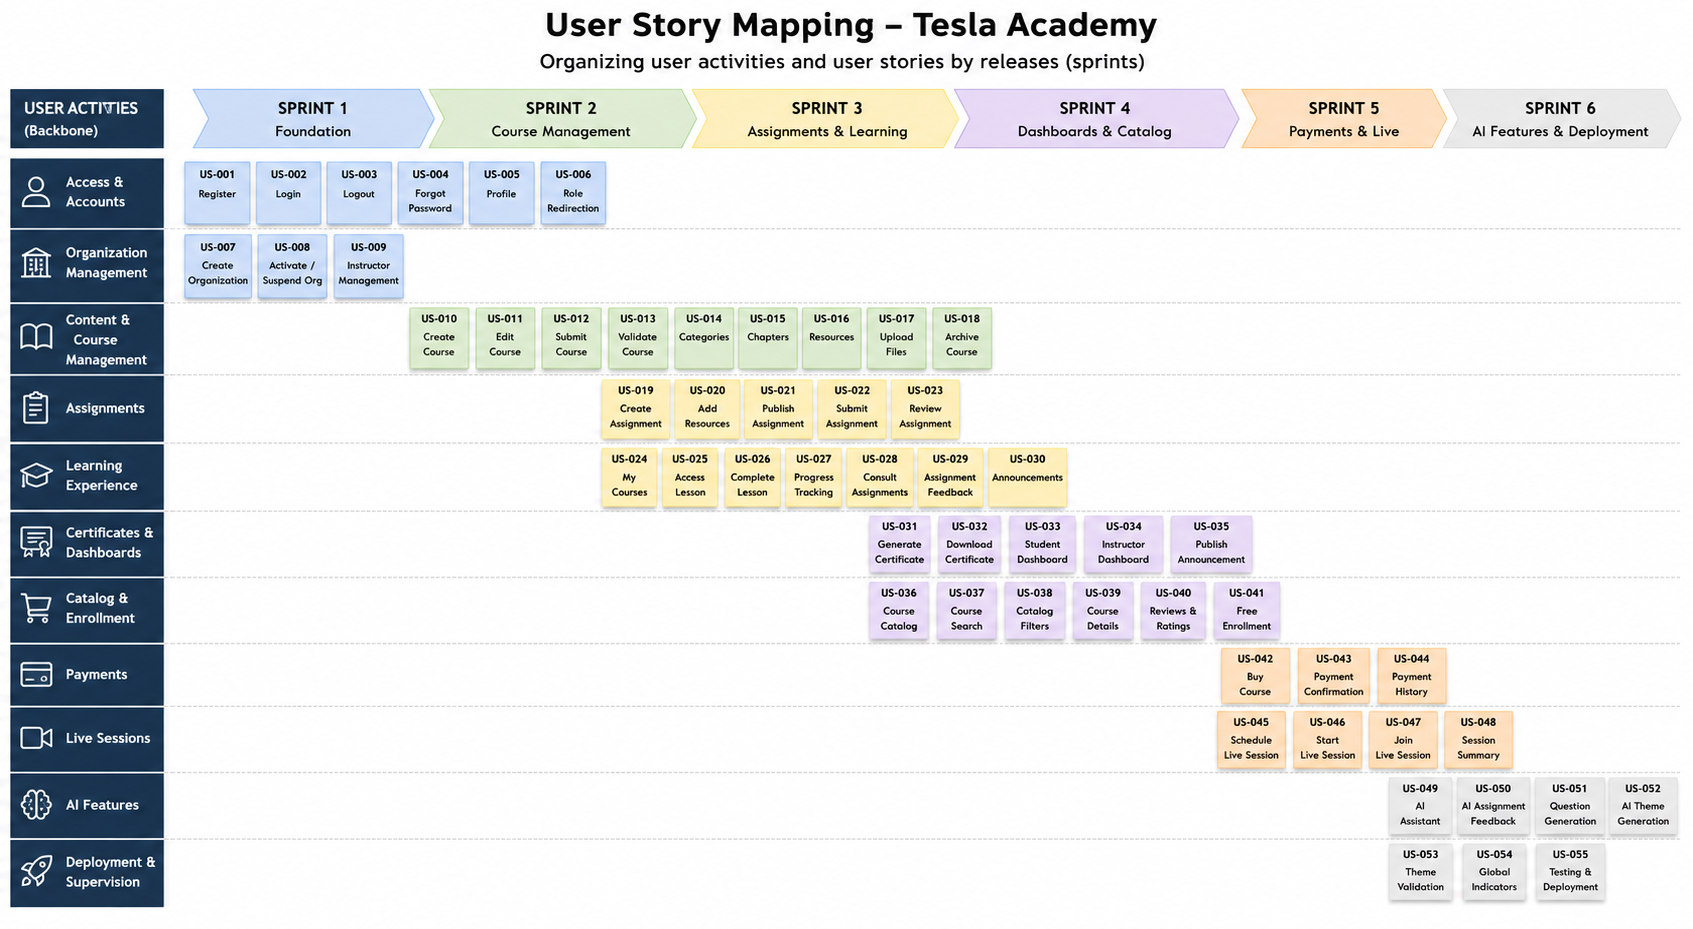
\includegraphics[width=\textwidth]{user_story_mapping.png}}
  \caption{User Story Mapping of Tesla Academy}
  \label{fig:user_story_mapping}
\end{figure}

The User Story Mapping organizes the main functionalities according to user activities and
planned releases. It provides a visual overview of the platform scope and helps prioritize
development according to the value delivered to users.

%% ----------------------------
\subsection{Release and Sprint Planning}
%% ----------------------------

Tesla Academy is planned in \textbf{3 releases} and \textbf{6 sprints}, with each sprint
lasting two weeks. The estimated total duration is therefore \textbf{12 weeks}.

Testing activities are integrated throughout all sprints. Each sprint ends with the
validation of the implemented features. The final sprint is dedicated to AI features,
global validation, deployment preparation, and final adjustments.

\begingroup
\footnotesize
\setlength{\tabcolsep}{4pt}

\begin{longtable}{|p{1.6cm}|p{2.2cm}|p{7.4cm}|p{2.2cm}|}
\caption{Release and Sprint Planning of Tesla Academy}
\label{tab:release_planning} \\
\hline
\textbf{Release} & \textbf{Sprint} & \textbf{Objective} & \textbf{US} \\
\hline
\endfirsthead

\hline
\textbf{Release} & \textbf{Sprint} & \textbf{Objective} & \textbf{US} \\
\hline
\endhead

\hline
\endfoot

\multicolumn{4}{|l|}{\textbf{Release 1 -- Foundation and Core Management}} \\
\hline
R1 & Sprint 1 & Authentication, user profile management, role-based access, organization creation, organization activation, and instructor management. & US-001--009 \\
\hline
R1 & Sprint 2 & Course creation, course editing, course validation, category management, chapter organization, resource management, file upload, and course archiving. & US-010--018 \\
\hline

\multicolumn{4}{|l|}{\textbf{Release 2 -- Learning Experience and Course Access}} \\
\hline
R2 & Sprint 3 & Assignment management, assignment submission, assignment review, lesson access, learner progress tracking, assignment feedback, and announcements. & US-019--030 \\
\hline
R2 & Sprint 4 & Certificate generation, dashboards, course catalog, course search, course filtering, course details, reviews, and free course enrollment. & US-031--041 \\
\hline

\multicolumn{4}{|l|}{\textbf{Release 3 -- Advanced Services and Deployment}} \\
\hline
R3 & Sprint 5 & Paid course purchase, payment confirmation, payment history, live session scheduling, live session start, live session access, and session summary. & US-042--048 \\
\hline
R3 & Sprint 6 & Contextual AI assistant, AI-assisted assignment feedback, question generation, AI theme generation, theme validation, global indicators, final validation, and deployment. & US-049--055 \\
\hline

\multicolumn{3}{|r|}{\textbf{Total -- 6 sprints -- 12 weeks}}
& \textbf{US-001--055} \\
\hline

\end{longtable}
\endgroup

%% ============================================================
\section{System Architecture and Design}
%% ============================================================

This section presents the overall design of the Tesla Academy platform, describing the
global system architecture, the selected technologies, and the database design that support
its implementation. The architectural choices are driven by the need for multi-tenancy,
security, scalability, maintainability, and seamless integration of AI-powered services.

%% ----------------------------
\subsection{Architecture Overview}
%% ----------------------------

Tesla Academy is designed as a distributed, multi-tier web application. The system is
composed of three main service layers: a \textbf{Next.js frontend}, an \textbf{Express.js
backend API}, and a dedicated \textbf{Python FastAPI AI service}. These layers communicate
through HTTP-based REST interfaces and rely on a shared PostgreSQL database and an
external object storage service.

\begin{figure}[H]
  \centerline{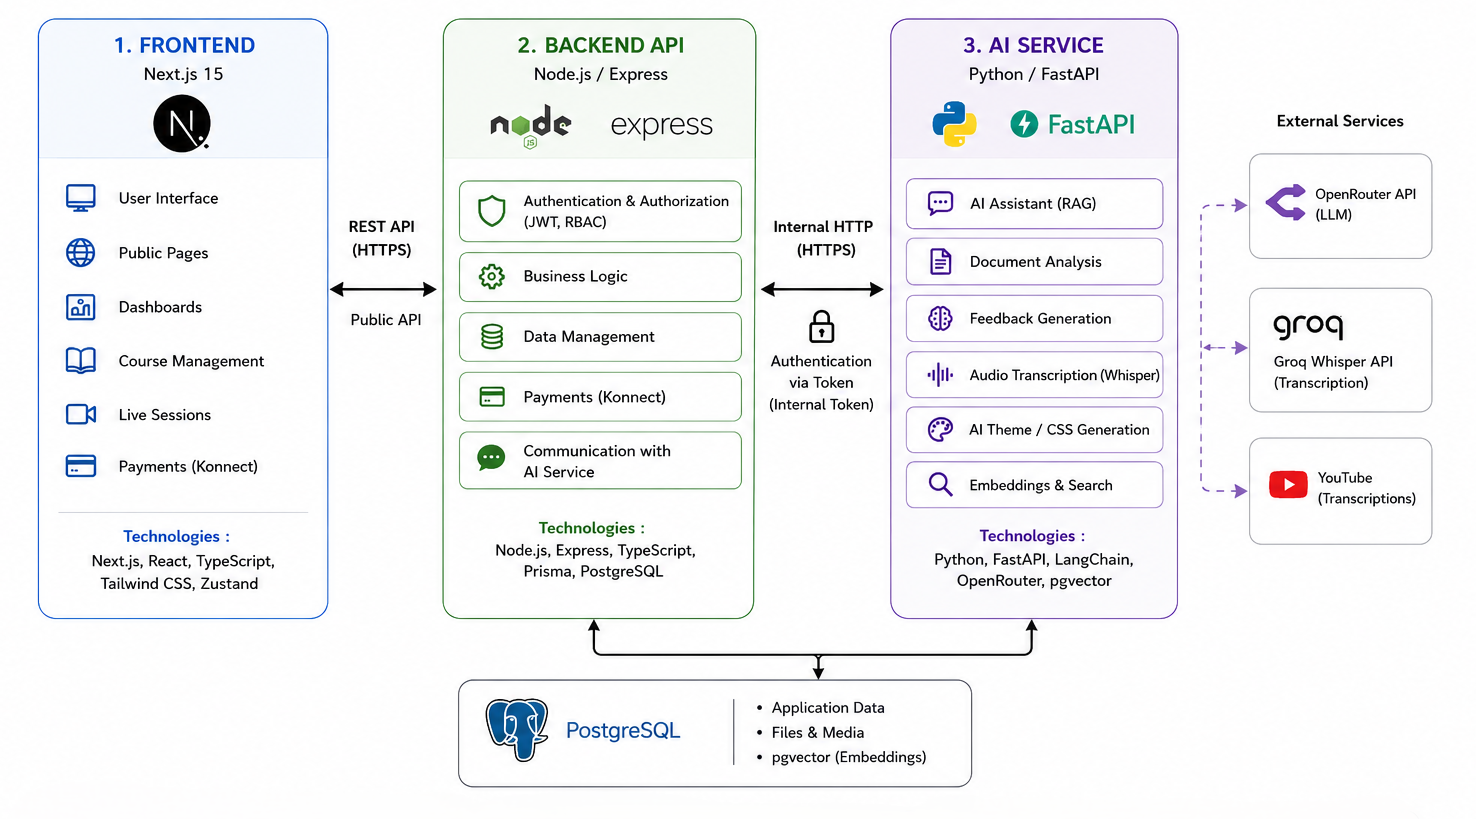
\includegraphics[width=0.85\textwidth]{global_architecture.png}}
  \caption{Global Architecture of Tesla Academy}
  \label{fig:global_architecture}
\end{figure}

%% ----------------------------
\subsection{Multi-Tenancy and Data Isolation}
%% ----------------------------

Tesla Academy is designed around a multi-tenant architecture. Several organizations can use
the same platform and infrastructure while keeping their data, users, courses, settings, and
activities logically isolated. The \texttt{Organization} entity is the root tenant of the
system; most organization-scoped entities carry an \texttt{organizationId} foreign key that
the backend uses to filter data and prevent cross-organization access.

\begin{figure}[H]
  \centerline{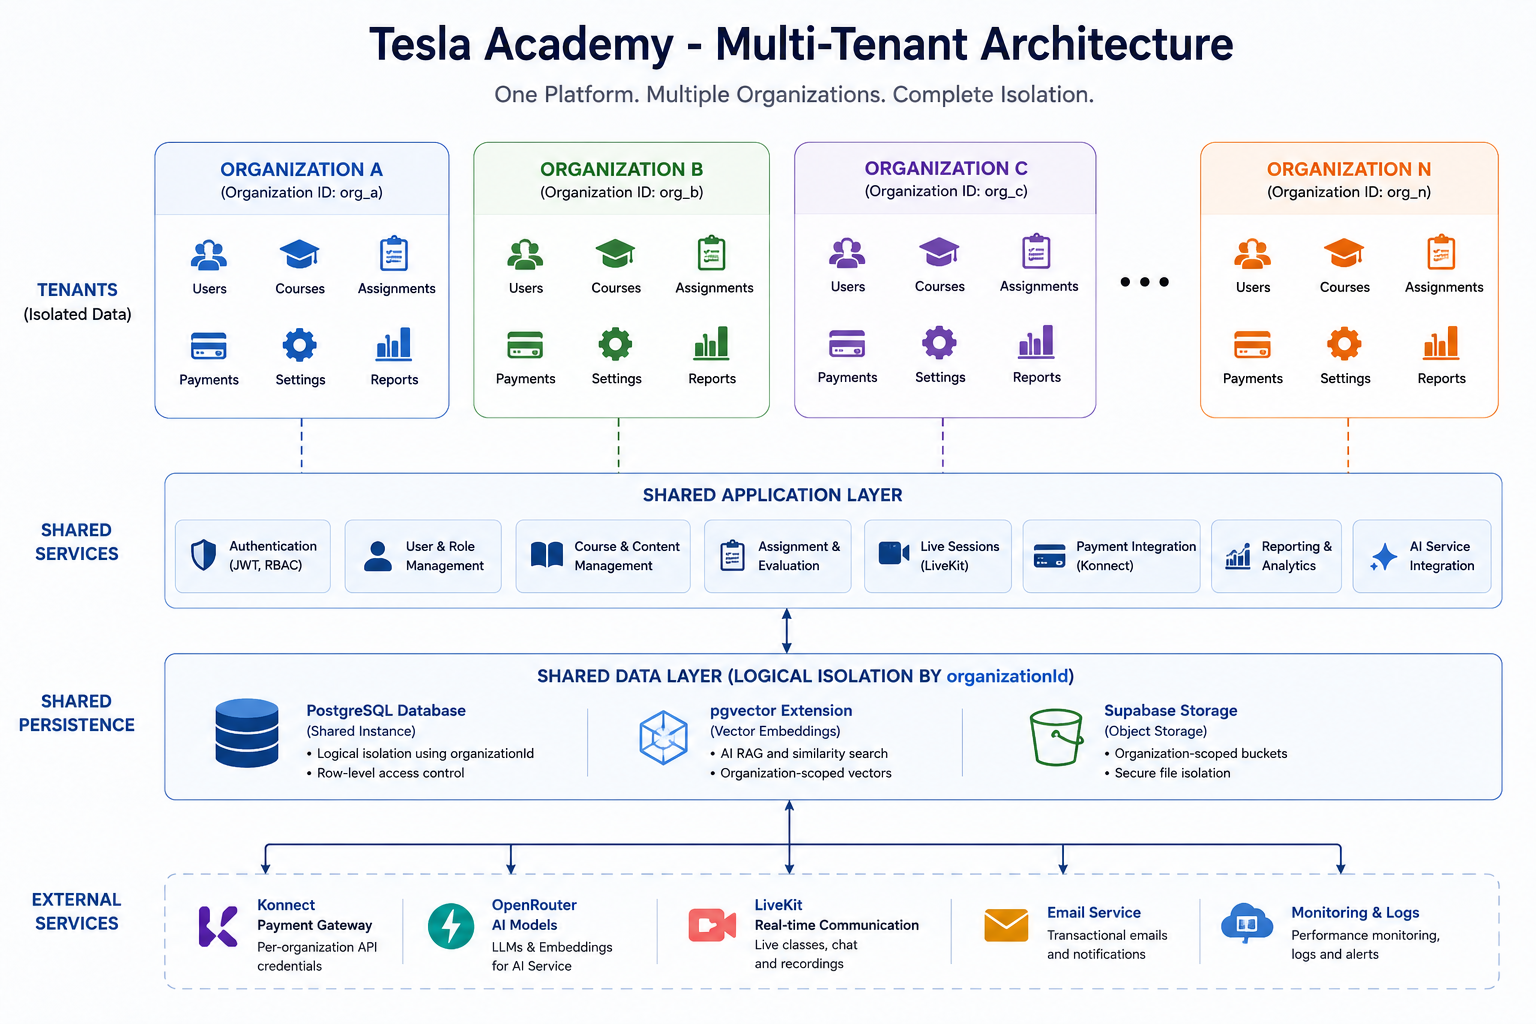
\includegraphics[width=0.75\textwidth]{Multi-Tenant_Architecture.png}}
  \caption{Multi-Tenant Architecture of Tesla Academy}
  \label{fig:Multi-Tenancy}
\end{figure}

This architecture provides data isolation per organization, shared infrastructure for all
tenants, organization-level customization of branding and AI settings, and the ability to
onboard new organizations without deploying separate instances.

%% ----------------------------
\subsection{Technology Stack}
%% ----------------------------

The following tables present the technologies used in each layer of the platform, along
with their respective roles.

\subsubsection{Frontend}

\begingroup
\small
\renewcommand{\arraystretch}{1.4}
\setlength{\tabcolsep}{6pt}
\begin{longtable}{|m{2.8cm}|p{11cm}|}
  \caption{Frontend Technologies}
  \label{tab:frontend_stack} \\
  \hline
  \textbf{Technology} & \textbf{Role and Description} \\
  \hline
  \endfirsthead
  \hline
  \textbf{Technology} & \textbf{Role and Description} \\
  \hline
  \endhead
  \hline
  \endfoot

  
\includegraphics[height=1cm]{nextjs-logo.jpg} &
  \textbf{Next.js / React} --- The frontend is developed with Next.js, a framework built
  on React. It provides routing, page loading optimization, and performance improvements.
  React enables the construction of reusable UI components for the admin, instructor, and
  student spaces. \\
  \hline
  
\includegraphics[height=1cm]{Tailwind_CSS_Logo.svg.png} &
  \textbf{Tailwind CSS / Radix UI / shadcn/ui} --- Tailwind CSS is used to create modern,
  responsive, and consistent interfaces. Radix UI and shadcn/ui provide accessible,
  reusable, and easily customizable components such as menus, forms, dialog boxes, and
  data tables. \\
  \hline
  \raisebox{0.2cm}{\textbf{TanStack}} &
  \textbf{TanStack Query / Zustand / TipTap} --- TanStack Query manages data exchanges
  between the frontend and the backend, facilitating loading, updating, and synchronizing
  displayed information. Zustand manages global application states such as session data and
  user preferences. TipTap serves as a rich text editor for creating and formatting
  educational content. \\
  \hline
  
\includegraphics[height=1cm]{videojs.png} &
  \textbf{Video.js} --- Used on the frontend to ensure smooth playback of video content
  and provide students with a seamless learning experience. \\
  \hline
\end{longtable}
\endgroup

\subsubsection{Backend API}

\begingroup
\small
\renewcommand{\arraystretch}{1.4}
\setlength{\tabcolsep}{6pt}
\begin{longtable}{|m{2.8cm}|p{11cm}|}
  \caption{Backend Technologies}
  \label{tab:backend_stack} \\
  \hline
  \textbf{Technology} & \textbf{Role and Description} \\
  \hline
  \endfirsthead
  \hline
  \textbf{Technology} & \textbf{Role and Description} \\
  \hline
  \endhead
  \hline
  \endfoot

  
\includegraphics[height=1cm]{nodejs_express_logo.png} &
  \textbf{Node.js / Express.js / TypeScript} --- The backend is developed with Node.js and
  Express.js, responsible for processing requests, applying business rules, and
  communicating with the platform's other services. TypeScript improves code quality,
  reduces development errors, and facilitates maintenance. Authentication, role-based
  authorization, data validation, and route protection strengthen API security. \\
  \hline
  
\includegraphics[height=1cm]{postgresql_supabase_logo.png} &
  \textbf{PostgreSQL / Supabase} --- PostgreSQL is used as the relational database
  management system, storing data related to users, courses, assessments, enrollments, and
  organizations. Supabase provides the database infrastructure and additional services,
  notably file storage. \\
  \hline
  
\includegraphics[height=1cm]{prisma_logo.png} &
  \textbf{Prisma ORM} --- Prisma facilitates interactions between the backend and
  PostgreSQL. It enables secure data manipulation, simplifies migration management, and
  produces more readable and maintainable data access code. \\
  \hline
\end{longtable}
\endgroup

\subsubsection{Artificial Intelligence Service}

\begingroup
\small
\renewcommand{\arraystretch}{1.4}
\setlength{\tabcolsep}{6pt}
\begin{longtable}{|m{2.8cm}|p{11cm}|}
  \caption{AI Service Technologies}
  \label{tab:ai_stack} \\
  \hline
  \textbf{Technology} & \textbf{Role and Description} \\
  \hline
  \endfirsthead
  \hline
  \textbf{Technology} & \textbf{Role and Description} \\
  \hline
  \endhead
  \hline
  \endfoot

  
\includegraphics[height=1cm]{astapi_python_logo.png} &
  \textbf{Python / FastAPI} --- The AI service is developed with Python and FastAPI,
  deployed independently of the main backend. Python was chosen for its extensive
  ecosystem of natural language processing libraries; FastAPI enables rapid development
  of high-performance, maintainable APIs. \\
  \hline
  
\includegraphics[height=1cm]{openrouter.png} &
  \textbf{OpenRouter} --- Used as a gateway to access the language models powering the
  platform, notably models from the DeepSeek family. This technology supports the
  intelligent assistant, question generation, automated feedback, and pedagogical
  assistance features. \\
  \hline
  
\includegraphics[height=1cm]{groq_logo.png} &
  \textbf{Groq Whisper / ffmpeg} --- Groq Whisper provides automatic transcription of
  audio and video content. ffmpeg handles media file processing and conversion before
  transcription when necessary. \\
  \hline
  \includegraphics[height=1cm]{pgvector_logo.png} &
  \textbf{pgvector} --- A PostgreSQL extension that enables semantic searches on
  educational resources, enhancing the intelligent assistant's ability to identify the most
  relevant content among available materials. \\
  \hline
\end{longtable}
\endgroup

\subsubsection{External Services}

\begingroup
\small
\renewcommand{\arraystretch}{1.4}
\setlength{\tabcolsep}{6pt}
\begin{longtable}{|m{2.8cm}|p{11cm}|}
  \caption{External Services}
  \label{tab:external_services} \\
  \hline
  \textbf{Technology} & \textbf{Role and Description} \\
  \hline
  \endfirsthead
  \hline
  \textbf{Technology} & \textbf{Role and Description} \\
  \hline
  \endhead
  \hline
  \endfoot

  
\includegraphics[height=1cm]{livekit_logo.png} &
  \textbf{LiveKit} --- Manages live training sessions by providing real-time audio and
  video communication between instructors and students, supporting synchronous interactions
  that complement the available educational resources. \\
  \hline
  
\includegraphics[height=1cm]{konnect_logo.png} &
  \textbf{Konnect} --- The payment gateway integrated into Tesla Academy, enabling users
  to make secure payments for course purchases and ensuring complete management of the
  payment process up to transaction validation. \\
  \hline
  \includegraphics[height=1cm]{supabase_storage_logo.png} &
  \textbf{Supabase Storage} --- Used for storing educational resources including videos,
  documents, and uploaded files, providing centralized and secure management of educational
  content. \\
  \hline
\end{longtable}
\endgroup

%% ----------------------------
\subsection{Development Tools}
%% ----------------------------

\begingroup
\small
\renewcommand{\arraystretch}{1.25}
\setlength{\tabcolsep}{4pt}
\begin{longtable}{|p{4cm}|p{3.5cm}|p{7cm}|}
\caption{Development Tools Used}
\label{tab:dev_tools} \\
\hline
\textbf{Category} & \textbf{Tool} & \textbf{Usage} \\
\hline
\endfirsthead
\hline
\textbf{Category} & \textbf{Tool} & \textbf{Usage} \\
\hline
\endhead
\hline
\endfoot
Development Environment & Visual Studio Code & Development of frontend, backend and AI service \\
\hline
Version Control & Git / GitHub & Source code management and version tracking \\
\hline
API Testing & Insomnia & Testing routes and API requests \\
\hline
Database & Prisma Studio & Data browsing and verification \\
\hline
Design & Figma & Creation of user interface mockups \\
\hline
Diagrams & draw.io & Creation of UML and architecture diagrams \\
\hline
Project Management & Notion & Task management and project tracking \\
\hline
\end{longtable}
\endgroup

%% ----------------------------
\subsection{Database Design}
%% ----------------------------

The data model of Tesla Academy is implemented as a relational schema in PostgreSQL and
managed through Prisma ORM. The schema is designed to support multi-tenancy through the
systematic use of \texttt{organizationId} foreign keys on organization-scoped entities.

\begin{figure}[H]
  \centerline{\includegraphics[width=\textwidth]{erd.png}}
  \caption{Entity Relationship Diagram of Tesla Academy}
  \label{fig:erd}
\end{figure}

The platform's data model is organized around the following principal entities:

\begin{itemize}

  \item \textbf{Organization and OrganizationConfig}: the root tenant entity, storing
        identification details such as name, slug, subdomain, and activation status, along
        with a configuration record that holds branding, payment parameters, AI provider
        settings, and feature flags for each organization.

  \item \textbf{User and Teacher}: users belong to an organization and carry a role
        (administrator, teacher, or student). The Teacher entity extends the user record
        with instructor-specific data linked to courses, assignments, and schedules.

  \item \textbf{Batch (Course) and Content Hierarchy}: a Batch represents a training
        course. Course content is organized hierarchically into Subjects, Chapters, Topics,
        and Content records (videos, PDFs, text blocks, or external links), allowing
        instructors to structure material into clear learning units.

  \item \textbf{Assignment and AssignmentSubmission}: an Assignment stores the title,
        instructions, deadline, and maximum mark. Each student response is recorded in an
        AssignmentSubmission, which holds the submitted text, attached files, status,
        grade, and optional AI-generated feedback.

  \item \textbf{BatchEnrollment and BatchCertificateIssue}: BatchEnrollment tracks which
        students are enrolled in which courses. BatchCertificateIssue records certificates
        awarded to students upon successful course completion, with a unique credential
        identifier and issue date.

  \item \textbf{Order}: records purchase transactions, storing buyer identity, purchased
        entity, amount, currency, payment provider reference, and payment status.

  \item \textbf{Schedule}: represents a scheduled live session, storing the title,
        date, duration, associated course, LiveKit room information, and optional
        transcription data used for post-session summarization.

  \item \textbf{Report}: stores generated analytics used by administrators to monitor
        platform activity, learning progress, payments, and AI-related usage.

\end{itemize}

%% ------------------------------------------------------------
\section*{Conclusion}
\addcontentsline{toc}{section}{Conclusion}
%% ------------------------------------------------------------

This chapter presented the requirements analysis, project planning, and system architecture
of Tesla Academy. It identified the main actors and their responsibilities, described the
functional and non-functional requirements, and introduced the general use case diagram.
The Scrum-based planning defined the Product Backlog, User Story Mapping, and a release
plan organized into three releases and six two-week sprints.

The chapter also described the global multi-service architecture, the technology stack
chosen to maximize productivity, type safety, and maintainability, and the relational
database design that supports the platform's multi-tenant and AI-powered requirements.
The next chapter focuses on the implementation of Release 1, covering authentication,
user management, organization management, and course structure functionalities.\include{chapter3_updated}%% ============================================================
%%  Chapter 5 — Release 2: Learning Experience and Course Access
%% ============================================================
\begingroup
\renewcommand{\baselinestretch}{0.85}
\chapter{Release 2: Learning Experience and Course Access}
\minitoc
\endgroup
\newpage

%% ------------------------------------------------------------
\section*{Introduction}
\addcontentsline{toc}{section}{Introduction}
%% ------------------------------------------------------------

With the foundational infrastructure established in Release 1, Release 2 shifts the
focus toward the student-facing dimension of the platform. While the first release
provided the tools necessary to create and structure educational content, this release
delivers the mechanisms through which students can discover, access, and progress
through that content. It represents the core of the learning experience that Tesla
Academy is designed to offer.

Release 2 corresponds to Sprints 3 and 4 of the project plan. Sprint 3 introduces the
assignment workflow, lesson access and completion tracking, progress measurement, and
student notifications. Sprint 4 extends the platform with certificate generation,
role-specific dashboards for both students and instructors, the public course catalog
with search and filtering capabilities, course reviews, and free course enrollment.

The chapter follows the same structure as the previous one: sprint backlog, functional
and technical specifications for all user stories, design models, and implementation
results.

%% ------------------------------------------------------------
\section{Sprint Backlog}
%% ------------------------------------------------------------

\begin{table}[H]
\centering
\caption{Sprint Backlog — Release 2}
\label{tab:backlog_r2}
\renewcommand{\arraystretch}{1.25}
\footnotesize
\begin{tabularx}{\textwidth}{|p{1.4cm}|p{1.5cm}|p{2.8cm}|p{6.8cm}|p{1.5cm}|}
\hline
\textbf{Sprint} & \textbf{Code} & \textbf{Feature} & \textbf{User Story} & \textbf{Est. (h)} \\
\hline
\multirow{12}{*}{Sprint 3}
  & US-019 & Assignment creation & Create an assignment with title, instructions, and deadline & 16 \\
  \cline{2-5}
  & US-020 & Assignment resources & Attach files and resources to an assignment & 8 \\
  \cline{2-5}
  & US-021 & Assignment publication & Publish an assignment to enrolled students & 8 \\
  \cline{2-5}
  & US-022 & Assignment submission & Submit an assignment response before the deadline & 16 \\
  \cline{2-5}
  & US-023 & Assignment review & Review submissions and provide feedback and grades & 16 \\
  \cline{2-5}
  & US-024 & My courses & View the list of enrolled courses & 8 \\
  \cline{2-5}
  & US-025 & Access lesson & Access lesson content such as videos and documents & 16 \\
  \cline{2-5}
  & US-026 & Complete lesson & Mark a lesson as completed & 8 \\
  \cline{2-5}
  & US-027 & Progress tracking & Track course progress percentage & 8 \\
  \cline{2-5}
  & US-028 & Consult assignments & View the list of assignments for enrolled courses & 8 \\
  \cline{2-5}
  & US-029 & Assignment feedback & Consult grades and feedback for submitted assignments & 8 \\
  \cline{2-5}
  & US-030 & Announcements & Consult announcements published by the instructor & 8 \\
\hline
\multirow{11}{*}{Sprint 4}
  & US-031 & Certificate generation & Obtain a certificate after completing a course & 16 \\
  \cline{2-5}
  & US-032 & Certificate download & Download the certificate in PDF format & 8 \\
  \cline{2-5}
  & US-033 & Student dashboard & View courses, progress, assignments, and certificates & 16 \\
  \cline{2-5}
  & US-034 & Instructor dashboard & Monitor course statistics and student submissions & 16 \\
  \cline{2-5}
  & US-035 & Publish announcement & Publish announcements for enrolled students & 8 \\
  \cline{2-5}
  & US-036 & Course catalog & View the list of available courses & 16 \\
  \cline{2-5}
  & US-037 & Course search & Search for a course by keyword & 8 \\
  \cline{2-5}
  & US-038 & Catalog filters & Filter courses by category, level, or price & 8 \\
  \cline{2-5}
  & US-039 & Course details & View detailed information about a course & 8 \\
  \cline{2-5}
  & US-040 & Reviews and ratings & Rate and comment on a completed course & 8 \\
  \cline{2-5}
  & US-041 & Free course enrollment & Enroll in a free course without payment & 8 \\
\hline
\end{tabularx}
\end{table}

%% ------------------------------------------------------------
\section{Functional and Technical Specifications}
%% ------------------------------------------------------------

This section provides a detailed breakdown of all user stories implemented in Release 2.
For each functional area, a specification table describes the user story, the associated
business rules, the technical implementation details, and the acceptance criteria that
were used to validate the delivered functionality.

%% ----------------------------
\subsection{Assignment Workflow (US-019 to US-023)}
%% ----------------------------

The assignment module introduces a structured assessment workflow involving three
actors: the instructor who creates and publishes assessments, the student who submits
responses, and the system which handles deadline enforcement and feedback notification.
The workflow supports multiple question types and accommodates both text-based and
file-based submission formats, providing instructors with flexible evaluation tools.

\begin{table}[H]
\centering
\caption{Specification — US-019: Assignment Creation}
\label{tab:us019}
\renewcommand{\arraystretch}{1.2}
\begin{tabularx}{\textwidth}{|p{3.5cm}|X|}
\hline
\textbf{User Story} & As an Instructor, I want to create an assignment with a title, instructions, and a deadline so that students have a clear and time-bound assessment task. \\
\hline
\textbf{Precondition} & The instructor is authenticated and owns at least one published course. \\
\hline
\textbf{Business Rules} &
\begin{itemize}[noitemsep, topsep=2pt]
  \item An assignment must be associated with an existing course;
  \item The assignment must include a title, instructions, and a deadline;
  \item Assignments are created in an unpublished state and are not visible to students until explicitly published.
\end{itemize} \\
\hline
\textbf{Technical Specification} &
\begin{itemize}[noitemsep, topsep=2pt]
  \item Assignments are stored in the \texttt{Assignment} model, linked to a \texttt{Batch} and scoped by \texttt{organizationId};
  \item Questions are stored in the \texttt{AssignmentQuestion} model and support four types: \texttt{QUIZ}, \texttt{TRUE\_FALSE}, \texttt{SHORT\_ANSWER}, and \texttt{FILE\_SUBMISSION};
  \item The deadline is stored as a timestamp and enforced by the backend at submission time.
\end{itemize} \\
\hline
\textbf{Acceptance Criteria} &
\begin{itemize}[noitemsep, topsep=2pt]
  \item The instructor can create an assignment with all required fields;
  \item The assignment is saved in unpublished state and not visible to students;
  \item Missing required fields are rejected with appropriate validation messages.
\end{itemize} \\
\hline
\end{tabularx}
\end{table}

\begin{table}[H]
\centering
\caption{Specification — US-020: Assignment Resources}
\label{tab:us020}
\renewcommand{\arraystretch}{1.2}
\begin{tabularx}{\textwidth}{|p{3.5cm}|X|}
\hline
\textbf{User Story} & As an Instructor, I want to attach files and supporting resources to an assignment so that students have all necessary material to complete their work. \\
\hline
\textbf{Precondition} & The assignment has been created and the instructor is authenticated. \\
\hline
\textbf{Business Rules} &
\begin{itemize}[noitemsep, topsep=2pt]
  \item Resources must be attached to an existing assignment;
  \item Supported resource types include documents and reference files;
  \item Resources remain accessible to enrolled students once the assignment is published.
\end{itemize} \\
\hline
\textbf{Technical Specification} &
\begin{itemize}[noitemsep, topsep=2pt]
  \item Attached files are uploaded to Supabase Storage via presigned URLs;
  \item File URLs are stored in the \texttt{Assignment} model as a JSON array;
  \item The backend validates ownership before accepting resource attachments.
\end{itemize} \\
\hline
\textbf{Acceptance Criteria} &
\begin{itemize}[noitemsep, topsep=2pt]
  \item The instructor can attach one or more files to an assignment;
  \item Attached resources are stored successfully and linked to the assignment;
  \item Students can access the resources once the assignment is published.
\end{itemize} \\
\hline
\end{tabularx}
\end{table}

\begin{table}[H]
\centering
\caption{Specification — US-021: Assignment Publication}
\label{tab:us021}
\renewcommand{\arraystretch}{1.2}
\begin{tabularx}{\textwidth}{|p{3.5cm}|X|}
\hline
\textbf{User Story} & As an Instructor, I want to publish an assignment so that enrolled students can view it and submit their responses. \\
\hline
\textbf{Precondition} & The assignment exists and contains at least one question. \\
\hline
\textbf{Business Rules} &
\begin{itemize}[noitemsep, topsep=2pt]
  \item An assignment must be explicitly published before students can access it;
  \item Publication is independent of the course publication state;
  \item A published assignment cannot be deleted if students have already submitted responses.
\end{itemize} \\
\hline
\textbf{Technical Specification} &
\begin{itemize}[noitemsep, topsep=2pt]
  \item The publication state is managed through a boolean field on the \texttt{Assignment} model;
  \item Student-facing endpoints filter assignments by publication status before returning results;
  \item The backend validates that the assignment contains at least one question before allowing publication.
\end{itemize} \\
\hline
\textbf{Acceptance Criteria} &
\begin{itemize}[noitemsep, topsep=2pt]
  \item The instructor can publish an assignment from the management interface;
  \item Published assignments appear in the student workspace;
  \item Unpublished assignments remain hidden from students.
\end{itemize} \\
\hline
\end{tabularx}
\end{table}

\begin{table}[H]
\centering
\caption{Specification — US-022: Assignment Submission}
\label{tab:us022}
\renewcommand{\arraystretch}{1.2}
\begin{tabularx}{\textwidth}{|p{3.5cm}|X|}
\hline
\textbf{User Story} & As a Student, I want to submit my assignment response with text or attached files before the deadline so that the instructor can evaluate my work. \\
\hline
\textbf{Precondition} & The student is enrolled in the course and the assignment is published with an active deadline. \\
\hline
\textbf{Business Rules} &
\begin{itemize}[noitemsep, topsep=2pt]
  \item Students can only submit if they are enrolled in the associated course;
  \item Submissions are rejected after the deadline has passed;
  \item A student can only submit one response per assignment.
\end{itemize} \\
\hline
\textbf{Technical Specification} &
\begin{itemize}[noitemsep, topsep=2pt]
  \item Submissions are stored in the \texttt{AssignmentSubmission} table;
  \item The \texttt{fileUrls} JSON field stores the URLs of uploaded attachment files;
  \item The backend validates enrollment and deadline before persisting the submission;
  \item File uploads follow the same presigned URL mechanism used elsewhere on the platform.
\end{itemize} \\
\hline
\textbf{Acceptance Criteria} &
\begin{itemize}[noitemsep, topsep=2pt]
  \item An enrolled student can submit a response before the deadline;
  \item Submissions after the deadline are rejected with an appropriate error;
  \item The submission is stored and visible to the instructor for review.
\end{itemize} \\
\hline
\end{tabularx}
\end{table}

\begin{table}[H]
\centering
\caption{Specification — US-023: Assignment Review}
\label{tab:us023}
\renewcommand{\arraystretch}{1.2}
\begin{tabularx}{\textwidth}{|p{3.5cm}|X|}
\hline
\textbf{User Story} & As an Instructor, I want to review student submissions and provide feedback and grades so that students can understand their performance. \\
\hline
\textbf{Precondition} & At least one student has submitted a response to the assignment. \\
\hline
\textbf{Business Rules} &
\begin{itemize}[noitemsep, topsep=2pt]
  \item Instructors can review all submissions for assignments within their courses;
  \item Each submission can receive a numeric grade and written feedback;
  \item A notification email is sent to the student upon grading.
\end{itemize} \\
\hline
\textbf{Technical Specification} &
\begin{itemize}[noitemsep, topsep=2pt]
  \item Grades and feedback are stored in the \texttt{marksAwarded} and \texttt{feedback} fields of the \texttt{AssignmentSubmission} record;
  \item An email notification is dispatched to the student upon saving the grade;
  \item The review interface is accessible only to instructors owning the associated course.
\end{itemize} \\
\hline
\textbf{Acceptance Criteria} &
\begin{itemize}[noitemsep, topsep=2pt]
  \item The instructor can view all submissions for an assignment;
  \item The instructor can assign a grade and written feedback to each submission;
  \item The student receives an email notification after grading.
\end{itemize} \\
\hline
\end{tabularx}
\end{table}

%% ----------------------------
\subsection{Learning Experience (US-024 to US-030)}
%% ----------------------------

The learning experience module covers all interactions a student has with enrolled
courses. It includes accessing the list of enrolled courses, navigating lesson content,
marking topics as complete, tracking progress, consulting assignment tasks and feedback,
and reading instructor announcements. These features collectively form the daily
learning workflow of a student on the platform.

\begin{table}[H]
\centering
\caption{Specification — US-024: My Courses}
\label{tab:us024}
\renewcommand{\arraystretch}{1.2}
\begin{tabularx}{\textwidth}{|p{3.5cm}|X|}
\hline
\textbf{User Story} & As a Student, I want to view the list of courses I am enrolled in so that I can easily navigate to my learning content. \\
\hline
\textbf{Precondition} & The student is authenticated and is enrolled in at least one course. \\
\hline
\textbf{Business Rules} &
\begin{itemize}[noitemsep, topsep=2pt]
  \item Only courses for which the student holds an active enrollment record are displayed;
  \item The list shows basic course information including title, progress, and instructor name.
\end{itemize} \\
\hline
\textbf{Technical Specification} &
\begin{itemize}[noitemsep, topsep=2pt]
  \item The backend queries \texttt{BatchEnrollment} records filtered by the authenticated student's identifier;
  \item Course progress is computed server-side and included in the response;
  \item Results are scoped by \texttt{organizationId} to enforce tenant isolation.
\end{itemize} \\
\hline
\textbf{Acceptance Criteria} &
\begin{itemize}[noitemsep, topsep=2pt]
  \item The student can view all their enrolled courses in a dedicated workspace section;
  \item Each course card displays the title, instructor, and current progress;
  \item Courses from other organizations are never displayed.
\end{itemize} \\
\hline
\end{tabularx}
\end{table}

\begin{table}[H]
\centering
\caption{Specification — US-025: Access Lesson}
\label{tab:us025}
\renewcommand{\arraystretch}{1.2}
\begin{tabularx}{\textwidth}{|p{3.5cm}|X|}
\hline
\textbf{User Story} & As a Student, I want to access lesson content such as videos, documents, and text so that I can follow the course material at my own pace. \\
\hline
\textbf{Precondition} & The student is enrolled in the course and the lesson belongs to a published course. \\
\hline
\textbf{Business Rules} &
\begin{itemize}[noitemsep, topsep=2pt]
  \item A student must be enrolled in a course to access any of its lesson content;
  \item Content types include uploaded videos, YouTube videos, PDF documents, rich-text blocks, and external links;
  \item Access to content files is controlled through the backend to prevent unauthorized downloads.
\end{itemize} \\
\hline
\textbf{Technical Specification} &
\begin{itemize}[noitemsep, topsep=2pt]
  \item The backend verifies enrollment before returning content URLs or data;
  \item Video files are served through Supabase Storage URLs;
  \item The lesson viewer renders each content type using its corresponding component on the frontend.
\end{itemize} \\
\hline
\textbf{Acceptance Criteria} &
\begin{itemize}[noitemsep, topsep=2pt]
  \item An enrolled student can access all lesson content within a published course;
  \item Non-enrolled users are denied access and redirected appropriately;
  \item All content types are rendered correctly in the lesson viewer.
\end{itemize} \\
\hline
\end{tabularx}
\end{table}

\begin{table}[H]
\centering
\caption{Specification — US-026 and US-027: Lesson Completion and Progress Tracking}
\label{tab:us026}
\renewcommand{\arraystretch}{1.2}
\begin{tabularx}{\textwidth}{|p{3.5cm}|X|}
\hline
\textbf{User Stories} & US-026: Complete lesson; US-027: Track course progress percentage. \\
\hline
\textbf{User Story} & As a Student, I want to mark lessons as completed and track my overall progress so that I can follow my advancement through the course. \\
\hline
\textbf{Precondition} & The student is enrolled in the course and has accessed the lesson content. \\
\hline
\textbf{Business Rules} &
\begin{itemize}[noitemsep, topsep=2pt]
  \item A student must explicitly mark a topic as complete;
  \item Course progress is computed as the ratio of completed topics to the total number of topics;
  \item Reaching 100\% completion is a prerequisite for certificate generation.
\end{itemize} \\
\hline
\textbf{Technical Specification} &
\begin{itemize}[noitemsep, topsep=2pt]
  \item Completion events are stored in the \texttt{ContentProgress} table, with fields for \texttt{topicId}, \texttt{userId}, and \texttt{completedAt};
  \item A dedicated endpoint (\texttt{POST /api/batches/:batchId/topics/:topicId/complete}) handles the completion request;
  \item The overall progress percentage is computed server-side and returned in the enrollment detail response.
\end{itemize} \\
\hline
\textbf{Acceptance Criteria} &
\begin{itemize}[noitemsep, topsep=2pt]
  \item The student can mark any topic as complete from the lesson viewer;
  \item The progress bar updates immediately after marking a topic;
  \item The dashboard displays the correct progress percentage for each enrolled course.
\end{itemize} \\
\hline
\end{tabularx}
\end{table}

\begin{table}[H]
\centering
\caption{Specification — US-028 and US-029: Consult Assignments and Feedback}
\label{tab:us028}
\renewcommand{\arraystretch}{1.2}
\begin{tabularx}{\textwidth}{|p{3.5cm}|X|}
\hline
\textbf{User Stories} & US-028: Consult assignments; US-029: Consult feedback. \\
\hline
\textbf{User Story} & As a Student, I want to view all assignments for my enrolled courses and consult the grades and feedback I have received so that I can follow my assessment results. \\
\hline
\textbf{Precondition} & The student is enrolled in the course and assignments have been published by the instructor. \\
\hline
\textbf{Business Rules} &
\begin{itemize}[noitemsep, topsep=2pt]
  \item Only published assignments belonging to enrolled courses are visible to the student;
  \item Feedback and grades are visible only after the instructor has reviewed the submission;
  \item Students can view the deadline, submission status, and feedback for each assignment.
\end{itemize} \\
\hline
\textbf{Technical Specification} &
\begin{itemize}[noitemsep, topsep=2pt]
  \item The backend returns assignments filtered by the student's enrollment and publication status;
  \item The \texttt{AssignmentSubmission} record is queried to retrieve the submission status, grade, and feedback;
  \item Results are scoped by \texttt{organizationId} to preserve tenant isolation.
\end{itemize} \\
\hline
\textbf{Acceptance Criteria} &
\begin{itemize}[noitemsep, topsep=2pt]
  \item The student can view the list of published assignments for all enrolled courses;
  \item After submission review, the student can access the assigned grade and written feedback;
  \item Assignments from non-enrolled courses are not displayed.
\end{itemize} \\
\hline
\end{tabularx}
\end{table}

\begin{table}[H]
\centering
\caption{Specification — US-030: Announcements}
\label{tab:us030}
\renewcommand{\arraystretch}{1.2}
\begin{tabularx}{\textwidth}{|p{3.5cm}|X|}
\hline
\textbf{User Story} & As a Student, I want to consult announcements published by my instructor so that I stay informed about course updates and important information. \\
\hline
\textbf{Precondition} & The student is enrolled in the course and the instructor has published at least one announcement. \\
\hline
\textbf{Business Rules} &
\begin{itemize}[noitemsep, topsep=2pt]
  \item Announcements are scoped to a specific course and visible only to enrolled students;
  \item Announcements are displayed in reverse chronological order.
\end{itemize} \\
\hline
\textbf{Technical Specification} &
\begin{itemize}[noitemsep, topsep=2pt]
  \item Announcements are stored in a dedicated model linked to the \texttt{Batch} and scoped by \texttt{organizationId};
  \item The backend filters announcements by enrollment and organization context before returning results.
\end{itemize} \\
\hline
\textbf{Acceptance Criteria} &
\begin{itemize}[noitemsep, topsep=2pt]
  \item The student can view all announcements published for their enrolled courses;
  \item Announcements from non-enrolled courses are not accessible;
  \item Announcements are displayed with their publication date and content.
\end{itemize} \\
\hline
\end{tabularx}
\end{table}

%% ----------------------------
\subsection{Certificates and Dashboards (US-031 to US-035)}
%% ----------------------------

This group of user stories introduces the tools through which students and instructors
can track and monitor platform activity at a high level. Certificate generation
formalizes course completion as a verifiable achievement, while the dashboards provide
consolidated views of learning progress, course statistics, and upcoming activities.

\begin{table}[H]
\centering
\caption{Specification — US-031 and US-032: Certificate Generation and Download}
\label{tab:us031}
\renewcommand{\arraystretch}{1.2}
\begin{tabularx}{\textwidth}{|p{3.5cm}|X|}
\hline
\textbf{User Stories} & US-031: Certificate generation; US-032: Certificate download. \\
\hline
\textbf{User Story} & As a Student, I want to obtain and download a certificate after completing a course so that I can share a formal proof of my achievement. \\
\hline
\textbf{Precondition} & The student has completed 100\% of the topics in an enrolled course. \\
\hline
\textbf{Business Rules} &
\begin{itemize}[noitemsep, topsep=2pt]
  \item A certificate is issued automatically when all course topics have been completed;
  \item Each certificate carries a unique \texttt{credentialId} for public verification;
  \item A student can only receive one certificate per course;
  \item The certificate is downloadable in PDF format at any time.
\end{itemize} \\
\hline
\textbf{Technical Specification} &
\begin{itemize}[noitemsep, topsep=2pt]
  \item The completion check is triggered server-side when a topic is marked complete;
  \item A \texttt{BatchCertificateIssue} record is created with the \texttt{credentialId}, \texttt{userId}, \texttt{batchId}, and \texttt{issuedAt} timestamp;
  \item PDF generation is performed server-side using course and student metadata;
  \item The public verification URL follows the format \texttt{/certificates/:credentialId}.
\end{itemize} \\
\hline
\textbf{Acceptance Criteria} &
\begin{itemize}[noitemsep, topsep=2pt]
  \item A certificate is automatically issued upon 100\% course completion;
  \item The student can view and download the certificate from their dashboard;
  \item The certificate includes the student name, course title, organization name, and completion date;
  \item The credential ID enables public online verification of the certificate.
\end{itemize} \\
\hline
\end{tabularx}
\end{table}

\begin{table}[H]
\centering
\caption{Specification — US-033: Student Dashboard}
\label{tab:us033}
\renewcommand{\arraystretch}{1.2}
\begin{tabularx}{\textwidth}{|p{3.5cm}|X|}
\hline
\textbf{User Story} & As a Student, I want to view a consolidated dashboard showing my enrolled courses, progress, upcoming assignments, and earned certificates so that I can manage my learning activities efficiently. \\
\hline
\textbf{Precondition} & The student is authenticated and has at least one enrollment record. \\
\hline
\textbf{Business Rules} &
\begin{itemize}[noitemsep, topsep=2pt]
  \item The dashboard aggregates data from enrollments, progress records, assignments, and certificates;
  \item Only data belonging to the authenticated student is displayed;
  \item The dashboard provides quick navigation to each enrolled course and active assignment.
\end{itemize} \\
\hline
\textbf{Technical Specification} &
\begin{itemize}[noitemsep, topsep=2pt]
  \item A dedicated dashboard endpoint aggregates enrollment, progress, assignment, and certificate data for the authenticated student;
  \item All queries are scoped by both \texttt{userId} and \texttt{organizationId};
  \item Upcoming deadlines are computed by filtering assignments where the deadline has not yet passed.
\end{itemize} \\
\hline
\textbf{Acceptance Criteria} &
\begin{itemize}[noitemsep, topsep=2pt]
  \item The student dashboard displays enrolled courses with their progress percentages;
  \item Upcoming assignment deadlines are visible and sorted chronologically;
  \item Earned certificates are accessible directly from the dashboard.
\end{itemize} \\
\hline
\end{tabularx}
\end{table}

\begin{table}[H]
\centering
\caption{Specification — US-034: Instructor Dashboard}
\label{tab:us034}
\renewcommand{\arraystretch}{1.2}
\begin{tabularx}{\textwidth}{|p{3.5cm}|X|}
\hline
\textbf{User Story} & As an Instructor, I want to monitor course statistics and student submissions from a dedicated dashboard so that I can track learner engagement and manage my assessment workload. \\
\hline
\textbf{Precondition} & The instructor is authenticated and owns at least one published course. \\
\hline
\textbf{Business Rules} &
\begin{itemize}[noitemsep, topsep=2pt]
  \item The dashboard displays statistics only for courses owned by the authenticated instructor;
  \item Submission counts include both pending and graded submissions;
  \item Average progress is computed across all enrolled students per course.
\end{itemize} \\
\hline
\textbf{Technical Specification} &
\begin{itemize}[noitemsep, topsep=2pt]
  \item A dedicated endpoint aggregates enrollment counts, average progress, and pending submission counts for each course owned by the instructor;
  \item All queries are scoped by \texttt{teacherId} and \texttt{organizationId};
  \item Pending submissions are identified by filtering \texttt{AssignmentSubmission} records where \texttt{marksAwarded} is null.
\end{itemize} \\
\hline
\textbf{Acceptance Criteria} &
\begin{itemize}[noitemsep, topsep=2pt]
  \item The instructor can view enrollment counts and average progress for each of their courses;
  \item Pending assignment submissions requiring review are highlighted;
  \item Statistics from courses owned by other instructors are not displayed.
\end{itemize} \\
\hline
\end{tabularx}
\end{table}

\begin{table}[H]
\centering
\caption{Specification — US-035: Publish Announcement}
\label{tab:us035}
\renewcommand{\arraystretch}{1.2}
\begin{tabularx}{\textwidth}{|p{3.5cm}|X|}
\hline
\textbf{User Story} & As an Instructor, I want to publish announcements for my enrolled students so that I can communicate course updates and important information effectively. \\
\hline
\textbf{Precondition} & The instructor is authenticated and owns at least one course with enrolled students. \\
\hline
\textbf{Business Rules} &
\begin{itemize}[noitemsep, topsep=2pt]
  \item Announcements are linked to a specific course and visible only to its enrolled students;
  \item Only the instructor who owns the course can publish announcements for it;
  \item Announcements are displayed to students in reverse chronological order.
\end{itemize} \\
\hline
\textbf{Technical Specification} &
\begin{itemize}[noitemsep, topsep=2pt]
  \item Announcements are stored in a model linked to the \texttt{Batch} and scoped by \texttt{organizationId};
  \item The backend validates that the authenticated instructor owns the referenced course before saving;
  \item Student-facing endpoints filter announcements by the student's enrollment records.
\end{itemize} \\
\hline
\textbf{Acceptance Criteria} &
\begin{itemize}[noitemsep, topsep=2pt]
  \item The instructor can create and publish an announcement for a specific course;
  \item Enrolled students can see the announcement in their course workspace;
  \item Announcements from courses the student is not enrolled in are not displayed.
\end{itemize} \\
\hline
\end{tabularx}
\end{table}

%% ----------------------------
\subsection{Course Catalog and Enrollment (US-036 to US-041)}
%% ----------------------------

The course catalog is the public-facing entry point of each organization's learning
space. It allows students to discover available courses, explore their content and
instructor information, and enroll directly. The catalog is fully scoped to the current
tenant, ensuring that students see only the courses published by their organization.
Free enrollment is handled as an immediate operation, while paid enrollment is deferred
to the payment workflow introduced in Release 3.

\begin{table}[H]
\centering
\caption{Specification — US-036: Course Catalog}
\label{tab:us036}
\renewcommand{\arraystretch}{1.2}
\begin{tabularx}{\textwidth}{|p{3.5cm}|X|}
\hline
\textbf{User Story} & As a Student, I want to view the list of available courses in my organization so that I can explore the learning offerings and choose courses to enroll in. \\
\hline
\textbf{Precondition} & The student is authenticated and belongs to an active organization. \\
\hline
\textbf{Business Rules} &
\begin{itemize}[noitemsep, topsep=2pt]
  \item The catalog displays only published courses belonging to the student's organization;
  \item Archived or draft courses are excluded from the catalog;
  \item Each course card shows the title, category, level, instructor name, and price.
\end{itemize} \\
\hline
\textbf{Technical Specification} &
\begin{itemize}[noitemsep, topsep=2pt]
  \item Catalog queries filter \texttt{Batch} records by \texttt{status = PUBLISHED} and \texttt{organizationId};
  \item The response includes aggregated enrollment counts and average ratings where available;
  \item Results are paginated to support large course catalogs.
\end{itemize} \\
\hline
\textbf{Acceptance Criteria} &
\begin{itemize}[noitemsep, topsep=2pt]
  \item The student can view all published courses in their organization;
  \item Draft and archived courses are not visible in the catalog;
  \item Each course card displays the relevant information clearly.
\end{itemize} \\
\hline
\end{tabularx}
\end{table}

\begin{table}[H]
\centering
\caption{Specification — US-037 and US-038: Course Search and Catalog Filters}
\label{tab:us037}
\renewcommand{\arraystretch}{1.2}
\begin{tabularx}{\textwidth}{|p{3.5cm}|X|}
\hline
\textbf{User Stories} & US-037: Course search; US-038: Catalog filters. \\
\hline
\textbf{User Story} & As a Student, I want to search for courses by keyword and filter results by category, level, or price so that I can quickly find courses that match my interests. \\
\hline
\textbf{Precondition} & The student is on the course catalog page. \\
\hline
\textbf{Business Rules} &
\begin{itemize}[noitemsep, topsep=2pt]
  \item Search applies to course titles and descriptions;
  \item Filters can be combined: category, level, and price range can be applied simultaneously;
  \item All search and filter results remain scoped to the student's organization.
\end{itemize} \\
\hline
\textbf{Technical Specification} &
\begin{itemize}[noitemsep, topsep=2pt]
  \item Full-text search is implemented via a Prisma \texttt{contains} query on the \texttt{title} and \texttt{description} fields;
  \item Filters are applied as additional \texttt{WHERE} conditions on the catalog query;
  \item Search and filter parameters are passed as query parameters to the catalog endpoint.
\end{itemize} \\
\hline
\textbf{Acceptance Criteria} &
\begin{itemize}[noitemsep, topsep=2pt]
  \item The student can search for courses by entering a keyword;
  \item The student can filter results by category, level, and price range;
  \item Search and filter results update dynamically and remain scoped to the organization.
\end{itemize} \\
\hline
\end{tabularx}
\end{table}

\begin{table}[H]
\centering
\caption{Specification — US-039: Course Details}
\label{tab:us039}
\renewcommand{\arraystretch}{1.2}
\begin{tabularx}{\textwidth}{|p{3.5cm}|X|}
\hline
\textbf{User Story} & As a Student, I want to view detailed information about a course so that I can make an informed decision before enrolling. \\
\hline
\textbf{Precondition} & The course is published and the student is browsing the catalog. \\
\hline
\textbf{Business Rules} &
\begin{itemize}[noitemsep, topsep=2pt]
  \item The detail page is publicly accessible to all authenticated users of the organization;
  \item It displays the course description, instructor information, content outline, enrollment count, and student reviews.
\end{itemize} \\
\hline
\textbf{Technical Specification} &
\begin{itemize}[noitemsep, topsep=2pt]
  \item The detail endpoint returns the full course metadata along with the content hierarchy summary, instructor profile, and aggregated reviews;
  \item The content outline lists subjects and chapters without exposing individual topic content to non-enrolled users.
\end{itemize} \\
\hline
\textbf{Acceptance Criteria} &
\begin{itemize}[noitemsep, topsep=2pt]
  \item The student can access the course detail page from the catalog;
  \item The page displays complete course information including description, instructor, and reviews;
  \item The content outline is visible but lesson content remains inaccessible without enrollment.
\end{itemize} \\
\hline
\end{tabularx}
\end{table}

\begin{table}[H]
\centering
\caption{Specification — US-040: Reviews and Ratings}
\label{tab:us040}
\renewcommand{\arraystretch}{1.2}
\begin{tabularx}{\textwidth}{|p{3.5cm}|X|}
\hline
\textbf{User Story} & As a Student, I want to rate and comment on a course I have completed so that I can share my experience with other learners. \\
\hline
\textbf{Precondition} & The student has completed the course and does not yet have a submitted review for it. \\
\hline
\textbf{Business Rules} &
\begin{itemize}[noitemsep, topsep=2pt]
  \item Only students who have completed the course can submit a review;
  \item Each student can submit only one review per course;
  \item Reviews include a star rating from 1 to 5 and an optional text comment.
\end{itemize} \\
\hline
\textbf{Technical Specification} &
\begin{itemize}[noitemsep, topsep=2pt]
  \item Reviews are stored in the \texttt{BatchReview} table, linked to the \texttt{Batch} and \texttt{User};
  \item The backend verifies course completion before accepting a review submission;
  \item Uniqueness is enforced by a composite constraint on \texttt{userId} and \texttt{batchId}.
\end{itemize} \\
\hline
\textbf{Acceptance Criteria} &
\begin{itemize}[noitemsep, topsep=2pt]
  \item A student who has completed a course can submit a rating and comment;
  \item A second review submission for the same course is rejected;
  \item Reviews appear on the course detail page and contribute to the average rating.
\end{itemize} \\
\hline
\end{tabularx}
\end{table}

\begin{table}[H]
\centering
\caption{Specification — US-041: Free Course Enrollment}
\label{tab:us041}
\renewcommand{\arraystretch}{1.2}
\begin{tabularx}{\textwidth}{|p{3.5cm}|X|}
\hline
\textbf{User Story} & As a Student, I want to enroll in a free course without payment so that I can start learning immediately. \\
\hline
\textbf{Precondition} & The student is authenticated, the course is published, its price is set to zero, and the student is not already enrolled. \\
\hline
\textbf{Business Rules} &
\begin{itemize}[noitemsep, topsep=2pt]
  \item Free enrollment is available only for courses with a price of zero;
  \item A student cannot enroll twice in the same course;
  \item Enrollment grants immediate access to all lesson content within the course.
\end{itemize} \\
\hline
\textbf{Technical Specification} &
\begin{itemize}[noitemsep, topsep=2pt]
  \item The enrollment endpoint verifies the course price before creating a \texttt{BatchEnrollment} record;
  \item For free courses, the record is created directly without initiating a payment flow;
  \item A uniqueness check on \texttt{userId} and \texttt{batchId} prevents duplicate enrollments.
\end{itemize} \\
\hline
\textbf{Acceptance Criteria} &
\begin{itemize}[noitemsep, topsep=2pt]
  \item The student can enroll in a free course with a single action;
  \item Enrollment is confirmed immediately and the course appears in the student's course list;
  \item Attempting to enroll a second time returns an appropriate error.
\end{itemize} \\
\hline
\end{tabularx}
\end{table}

%% ------------------------------------------------------------
\section{Design}
%% ------------------------------------------------------------

The realization of Release 2 relies on the architectural foundations presented in
Chapter~3 and extends the data model introduced in Release 1. The following UML
models focus on the entities and interaction flows specific to this release.

\subsection{Static Modeling}

\subsubsection{Class Diagram}

Figure~\ref{fig:class_r2} presents the class diagram for Release 2. It extends the
data model of Release 1 by introducing the entities that support the learning
experience: assignments, content progress, enrollments, certificates, and reviews.
These entities collectively describe the relationship between a student and the courses
they interact with throughout their learning journey.

\begin{figure}[H]
  \centerline{\includegraphics[width=\textwidth]{class_diagram_r2.png}}
  \caption{Class Diagram — Release 2}
  \label{fig:class_r2}
\end{figure}

The main relationships introduced in this release are as follows:

\begin{itemize}
  \item A \texttt{BatchEnrollment} links a \texttt{User} (student) to a \texttt{Batch}
        (course) and serves as the gateway to all learning activities. Without an active
        enrollment record, a student cannot access any of the associated lessons,
        assignments, or certificates;
  \item A \texttt{ContentProgress} record tracks whether a student has completed a
        specific \texttt{Topic}, enabling the server-side computation of the overall
        course progress percentage;
  \item An \texttt{Assignment} belongs to a \texttt{Batch} and is composed of multiple
        \texttt{AssignmentQuestion} items; each enrolled student produces one
        \texttt{AssignmentSubmission} per assignment;
  \item A \texttt{BatchCertificateIssue} is automatically created by the backend when a
        student has completed all topics in their enrolled course, formalizing the
        achievement with a unique and verifiable credential identifier;
  \item A \texttt{BatchReview} records the student's rating and comment following course
        completion, contributing to the course quality indicators visible in the catalog.
\end{itemize}

\subsubsection{Database Model of Release 2}

Figure~\ref{fig:db_model_r2} presents the simplified database model for Release 2,
highlighting the new tables introduced to support the learning experience. It extends
the model of Release 1 with the enrollment, progress tracking, assignment, submission,
certificate, and review entities.

\begin{figure}[H]
  \centerline{\includegraphics[width=0.95\textwidth]{database_model_r2.png}}
  \caption{Database Model — Release 2}
  \label{fig:db_model_r2}
\end{figure}

\subsection{Dynamic Modeling}

The dynamic models of Release 2 focus on the three most significant interaction flows
from the student perspective: lesson access and completion, assignment submission, and
catalog browsing with enrollment.

\subsubsection{Lesson Access and Completion Sequence Diagram}

Figure~\ref{fig:seq_lesson} illustrates the sequence of interactions when a student
accesses a lesson and marks it as complete. Before returning any content, the backend
verifies that the student holds an active enrollment in the course. Upon successful
verification, the lesson resource is served. When the student explicitly marks the
topic as complete, the backend records the progress event in the \texttt{ContentProgress}
table and evaluates whether all topics in the course have been completed. If so, the
certificate issuance process is triggered automatically.

\begin{figure}[H]
  \centerline{\includegraphics[width=0.9\textwidth]{seq_lesson_completion.png}}
  \caption{Lesson Access and Completion Sequence Diagram}
  \label{fig:seq_lesson}
\end{figure}

\subsubsection{Assignment Submission Sequence Diagram}

Figure~\ref{fig:seq_assignment} illustrates the assignment submission flow from the
student's perspective. After selecting an assignment, the student fills in their
response and submits it before the configured deadline. The backend validates both the
enrollment status and the submission deadline before persisting the record. Once the
instructor reviews the submission and assigns a grade, the student is automatically
notified by email and can consult the feedback from their dashboard.

\begin{figure}[H]
  \centerline{\includegraphics[width=0.9\textwidth]{seq_assignment_submission.png}}
  \caption{Assignment Submission Sequence Diagram}
  \label{fig:seq_assignment}
\end{figure}

\subsubsection{Course Catalog and Free Enrollment Sequence Diagram}

Figure~\ref{fig:seq_catalog} illustrates the flow from catalog browsing to free course
enrollment. The student navigates to the catalog, which returns only the published
courses scoped to their organization. After applying optional filters and selecting a
course to view its details, the student clicks the enrollment button. For courses with
a price of zero, the backend creates the \texttt{BatchEnrollment} record immediately
and redirects the student to the course viewer without initiating a payment flow.

\begin{figure}[H]
  \centerline{\includegraphics[width=0.9\textwidth]{seq_catalog_enrollment.png}}
  \caption{Course Catalog and Free Enrollment Sequence Diagram}
  \label{fig:seq_catalog}
\end{figure}

%% ------------------------------------------------------------
\section{Implementation}
%% ------------------------------------------------------------

This section presents the implementation results of Release 2. Each subsection
describes one delivered functional module and is supported by interface screenshots
that illustrate the final state of the feature.

\subsection{Assignment Management}

The assignment module provides instructors with a comprehensive assessment creation
tool supporting four question types: multiple choice, true/false, short answer, and
file submission. Instructors can attach supporting resources to an assignment and
control its visibility independently of the course publication state, publishing it
only when the content is ready for students.

On the student side, the submission interface presents each assignment question in
sequence and allows the student to provide text answers or upload files as required.
The instructor's review interface consolidates all received submissions and provides
a grading panel where marks and written feedback can be entered directly. Upon
grading, the student receives an email notification and can consult the instructor's
feedback from their personal dashboard.

\begin{figure}[H]
  \centerline{\includegraphics[width=\textwidth]{screenshot_assignment_editor.png}}
  \caption{Assignment Editor — Instructor View}
  \label{fig:sc_assignment_editor}
\end{figure}

\begin{figure}[H]
  \centerline{\includegraphics[width=\textwidth]{screenshot_assignment_submission.png}}
  \caption{Assignment Submission — Student View}
  \label{fig:sc_assignment_submission}
\end{figure}

\subsection{Lesson Viewer and Progress Tracking}

The lesson viewer provides a unified interface for all supported content types.
Uploaded video files and YouTube-embedded videos are displayed in an adaptive video
player, while PDF documents are rendered inline using a browser-native renderer.
Rich-text content is displayed from stored HTML, and external links open in a new
browser tab. At the bottom of each lesson page, a completion button allows the student
to explicitly mark the topic as done, which immediately updates the course progress
bar and persists the completion event on the server.

\begin{figure}[H]
  \centerline{\includegraphics[width=\textwidth]{screenshot_lesson_viewer.png}}
  \caption{Lesson Viewer and Progress Bar — Student View}
  \label{fig:sc_lesson}
\end{figure}

\subsection{Student and Instructor Dashboards}

The student dashboard serves as a personal learning hub, consolidating in one view
the list of enrolled courses with their current progress percentages, upcoming
assignment deadlines, recent instructor announcements, and earned certificates. This
centralized overview allows students to manage their learning activities efficiently
without navigating between multiple sections of the platform.

The instructor dashboard is oriented toward monitoring and supervision. It presents
course-level statistics including total enrollment counts, average student progress,
and the number of assignment submissions awaiting review. This information enables
instructors to quickly identify courses that require attention and prioritize their
grading activities.

\begin{figure}[H]
  \centerline{\includegraphics[width=\textwidth]{screenshot_student_dashboard.png}}
  \caption{Student Dashboard}
  \label{fig:sc_student_dashboard}
\end{figure}

\begin{figure}[H]
  \centerline{\includegraphics[width=\textwidth]{screenshot_instructor_dashboard.png}}
  \caption{Instructor Dashboard}
  \label{fig:sc_instructor_dashboard}
\end{figure}

\subsection{Course Catalog}

The course catalog presents students with a browsable and searchable listing of all
published courses within their organization. Each course card displays the title,
category, difficulty level, instructor name, enrollment count, and price at a glance.
A filter sidebar allows students to narrow results by category and level, while the
search bar performs live filtering on the course title. The tenant isolation mechanism
ensures that each student sees only the courses belonging to their own organization.

\begin{figure}[H]
  \centerline{\includegraphics[width=\textwidth]{screenshot_catalog.png}}
  \caption{Course Catalog — Student View}
  \label{fig:sc_catalog}
\end{figure}

\subsection{Certificate Generation}

Upon completing all topics of an enrolled course, the platform automatically issues a
digital certificate to the student. The certificate document includes the student's
full name, the course title, the organization name, the date of completion, and a
unique credential identifier that can be used for public online verification. The
certificate is accessible from the student dashboard and can be downloaded at any
time in PDF format, providing students with a portable and shareable record of their
achievement.

\begin{figure}[H]
  \centerline{\includegraphics[width=\textwidth]{screenshot_certificate.png}}
  \caption{Certificate — Student View}
  \label{fig:sc_certificate}
\end{figure}

%% ------------------------------------------------------------
\section*{Conclusion}
\addcontentsline{toc}{section}{Conclusion}
%% ------------------------------------------------------------

This chapter presented the implementation of Release 2 of Tesla Academy, which
delivers the complete student-facing learning experience. Students can now discover
courses through the catalog, enroll in free offerings, access multimedia lesson content,
track their progress through the platform, submit assignments and receive instructor
feedback, and obtain verifiable digital certificates upon course completion.
Role-specific dashboards for both students and instructors provide consolidated views
of platform activity and support informed decision-making throughout the learning cycle.

The next chapter presents Release 3, which extends the platform with paid course
purchases via the Konnect payment gateway, live session management powered by
LiveKit, and AI-powered features including the contextual learning assistant,
AI-assisted assignment feedback, automatic question generation, and dynamic theme
generation.%% ============================================================
%%  Chapter 6 — Release 3: Advanced Services and AI Features
%% ============================================================
\begingroup
\renewcommand{\baselinestretch}{0.85}
\chapter{Release 3: Advanced Services and AI Features}
\minitoc
\endgroup
\newpage

%% ------------------------------------------------------------
\section*{Introduction}
\addcontentsline{toc}{section}{Introduction}
%% ------------------------------------------------------------

This chapter presents the implementation of the third and final release of Tesla Academy.
Release 3 corresponds to Sprints 5 and 6 and introduces the advanced services that
differentiate the platform from conventional LMS solutions: online payment processing,
live session management, and a comprehensive suite of AI-powered educational features.

Sprint 5 covers paid course purchases, payment verification, payment history, and live
session scheduling, start, and participation. Sprint 6 introduces the contextual AI
learning assistant, AI-assisted assignment feedback, automatic question generation,
AI-powered visual theme generation, global platform indicators for the Super Administrator,
and the final platform validation and deployment.

%% ------------------------------------------------------------
\section{Sprint Backlog}
%% ------------------------------------------------------------

\begin{table}[H]
\centering
\caption{Sprint Backlog — Release 3}
\label{tab:backlog_r3}
\renewcommand{\arraystretch}{1.25}
\footnotesize
\begin{tabularx}{\textwidth}{|p{1.4cm}|p{1.5cm}|p{2.8cm}|p{6.8cm}|p{1.5cm}|}
\hline
\textbf{Sprint} & \textbf{Code} & \textbf{Feature} & \textbf{User Story} & \textbf{Est. (h)} \\
\hline
\multirow{7}{*}{Sprint 5}
  & US-042 & Buy course & Purchase a paid course from the platform & 24 \\
  \cline{2-5}
  & US-043 & Payment confirmation & Confirm payment and activate course enrollment & 16 \\
  \cline{2-5}
  & US-044 & Payment history & Consult payment history & 8 \\
  \cline{2-5}
  & US-045 & Schedule live session & Schedule a live session with date, time, and duration & 16 \\
  \cline{2-5}
  & US-046 & Start live session & Start a live session using the live session service & 16 \\
  \cline{2-5}
  & US-047 & Join live session & Join a live session from the student workspace & 8 \\
  \cline{2-5}
  & US-048 & Automatic session summary & Generate a summary after a live session & 16 \\
\hline
\multirow{7}{*}{Sprint 6}
  & US-049 & Contextual AI assistant & Ask the AI assistant questions related to course content & 24 \\
  \cline{2-5}
  & US-050 & Assignment feedback with AI & Receive AI-assisted feedback on assignments & 16 \\
  \cline{2-5}
  & US-051 & Question generation & Generate quiz questions automatically & 16 \\
  \cline{2-5}
  & US-052 & AI theme generation & Generate a visual theme from a text description & 16 \\
  \cline{2-5}
  & US-053 & Theme validation & Validate the generated theme before applying it & 8 \\
  \cline{2-5}
  & US-054 & Global indicators & Consult global platform indicators & 16 \\
  \cline{2-5}
  & US-055 & Final validation and deployment & Perform final validation and deploy the platform & 16 \\
\hline
\end{tabularx}
\end{table}

%% ------------------------------------------------------------
\section{Functional and Technical Specifications}
%% ------------------------------------------------------------

\subsection{Payment Processing (US-042, US-043, US-044)}

\begin{table}[H]
\centering
\caption{Specification — Paid Course Purchase}
\label{tab:payment_spec}
\renewcommand{\arraystretch}{1.2}
\begin{tabularx}{\textwidth}{|p{3.5cm}|X|}
\hline
\textbf{User Stories} & US-042, US-043, US-044 — Course purchase, payment confirmation, payment history. \\
\hline
\textbf{Business Rules} &
\begin{itemize}[noitemsep, topsep=2pt]
  \item Paid course enrollment requires a successful payment transaction;
  \item Two payment providers are supported: \textbf{Konnect} and \textbf{Flouci},
        both supporting Tunisian Dinar (TND);
  \item Each organization configures its own payment credentials in its
        \texttt{OrganizationConfig};
  \item Payment amounts are expressed in millimes (1 TND = 1000 millimes);
  \item An \texttt{Order} record is created upon checkout initiation with status
        \texttt{PENDING}, and updated to \texttt{SUCCESS} or \texttt{FAILED} after
        payment gateway callback verification;
  \item Upon confirmed payment, the student is automatically enrolled in the purchased
        course via a \texttt{BatchEnrollment} record.
\end{itemize} \\
\hline
\textbf{Technical Specification} &
\begin{itemize}[noitemsep, topsep=2pt]
  \item Konnect integration uses the \texttt{/payments/init-payment} API endpoint to
        generate a payment URL; verification is performed via the
        \texttt{/payments/:ref} endpoint;
  \item Flouci integration uses a public/private key pair stored per organization;
  \item The payment mode is determined by the \texttt{paymentMode} field in
        \texttt{OrganizationConfig}: \texttt{per\_course} or \texttt{subscription};
  \item Callback URLs include the \texttt{orderId} parameter, allowing the backend to
        match and update the corresponding \texttt{Order} record;
  \item Enrollment is granted by the \texttt{grantOrderEntitlements} function only after
        payment status is confirmed as \texttt{SUCCESS}.
\end{itemize} \\
\hline
\textbf{Acceptance Criteria} &
\begin{itemize}[noitemsep, topsep=2pt]
  \item A student can initiate checkout for a paid course;
  \item After successful payment, the student is enrolled and can access course content;
  \item A failed or cancelled payment does not grant enrollment;
  \item The student can view their payment history from their dashboard.
\end{itemize} \\
\hline
\end{tabularx}
\end{table}

\subsection{Live Session Management (US-045 to US-048)}

\begin{table}[H]
\centering
\caption{Specification — Live Sessions}
\label{tab:livekit_spec}
\renewcommand{\arraystretch}{1.2}
\begin{tabularx}{\textwidth}{|p{3.5cm}|X|}
\hline
\textbf{User Stories} & US-045 to US-048 — Schedule, start, join, and summarize live sessions. \\
\hline
\textbf{Business Rules} &
\begin{itemize}[noitemsep, topsep=2pt]
  \item An instructor schedules a session by providing a title, course association,
        date, time, and expected duration;
  \item Enrolled students receive an email notification when a new session is scheduled;
  \item The instructor starts the session from their workspace, which transitions the
        \texttt{Schedule} status to \texttt{LIVE} and issues a host-role LiveKit token;
  \item Students join using a participant-role token; they can view and hear but cannot
        publish audio/video by default unless the host grants permission;
  \item After the session ends, if transcription data is available, the AI microservice
        automatically generates a structured summary of the session.
\end{itemize} \\
\hline
\textbf{Technical Specification} &
\begin{itemize}[noitemsep, topsep=2pt]
  \item Live sessions use \textbf{LiveKit}, an open-source WebRTC infrastructure;
  \item A \texttt{LiveKit JWT token} is generated server-side using the
        \texttt{LIVEKIT\_API\_KEY} and \texttt{LIVEKIT\_API\_SECRET} environment
        variables;
  \item Host tokens carry \texttt{canPublish: true} and \texttt{canSubscribe: true};
        student tokens carry \texttt{canPublish: false};
  \item Session transcription is collected incrementally on the client and sent to the
        backend after the session ends via the \texttt{transcriptDraft} field;
  \item The AI summarization endpoint (\texttt{POST /internal/v1/schedules/summarize})
        receives the transcript and returns a structured summary stored in the
        \texttt{aiSummary} field of the \texttt{Schedule} record;
  \item A collaborative whiteboard is available per session via the
        \texttt{ScheduleWhiteboard} entity.
\end{itemize} \\
\hline
\textbf{Acceptance Criteria} &
\begin{itemize}[noitemsep, topsep=2pt]
  \item An instructor can schedule and start a session; students can join using the
        provided room token;
  \item Session participants can communicate in real time;
  \item After the session, a summary is automatically generated and displayed;
  \item Completed sessions cannot be restarted.
\end{itemize} \\
\hline
\end{tabularx}
\end{table}

\subsection{Contextual AI Assistant (US-049)}

\begin{table}[H]
\centering
\caption{Specification — Contextual AI Assistant (RAG Chat)}
\label{tab:rag_spec}
\renewcommand{\arraystretch}{1.2}
\begin{tabularx}{\textwidth}{|p{3.5cm}|X|}
\hline
\textbf{User Story} & US-049 — As a student, I want to ask the AI assistant questions about course content so that I can get contextual explanations. \\
\hline
\textbf{Business Rules} &
\begin{itemize}[noitemsep, topsep=2pt]
  \item The AI assistant is scoped to the content of the course the student is
        currently viewing;
  \item Responses are grounded in the indexed course content through RAG;
  \item Each organization uses its own OpenRouter API key for AI calls;
  \item Conversation history is maintained within the session for multi-turn coherence.
\end{itemize} \\
\hline
\textbf{Technical Specification} &
\begin{itemize}[noitemsep, topsep=2pt]
  \item When educational content (YouTube video, PDF, text) is published, the backend
        triggers the \texttt{POST /internal/v1/content/index} endpoint to extract text
        and store vector embeddings in the \texttt{content\_embeddings} pgvector table;
  \item When the student sends a message, the AI microservice computes a query
        embedding, retrieves the top-$k$ most similar content chunks via cosine
        similarity, and injects them into the system prompt;
  \item The language model call is made through OpenRouter using the configured model
        (default: \texttt{google/gemini-flash-1.5});
  \item The response includes metadata: \texttt{ragChunksUsed} and \texttt{ragStatus},
        allowing the frontend to indicate whether retrieval was successful.
\end{itemize} \\
\hline
\textbf{Acceptance Criteria} &
\begin{itemize}[noitemsep, topsep=2pt]
  \item A student can ask a question and receive a contextually relevant answer;
  \item The assistant references information from the indexed course content;
  \item The conversation history is maintained within the session.
\end{itemize} \\
\hline
\end{tabularx}
\end{table}

\subsection{AI-Assisted Assignment Feedback (US-050)}

\begin{table}[H]
\centering
\caption{Specification — AI Assignment Feedback}
\label{tab:ai_feedback_spec}
\renewcommand{\arraystretch}{1.2}
\begin{tabularx}{\textwidth}{|p{3.5cm}|X|}
\hline
\textbf{User Story} & US-050 — As a student, I want to receive automatic AI-assisted feedback on my assignment so that I can understand my mistakes. \\
\hline
\textbf{Business Rules} &
\begin{itemize}[noitemsep, topsep=2pt]
  \item AI feedback is generated automatically when a student submits an assignment;
  \item The feedback analyzes each question response against the correct answer and
        the defined evaluation criteria;
  \item AI feedback is stored alongside the submission and displayed to the student;
  \item AI feedback does not replace the instructor's grade; it is supplementary.
\end{itemize} \\
\hline
\textbf{Technical Specification} &
\begin{itemize}[noitemsep, topsep=2pt]
  \item Upon submission, the backend compiles a structured prompt containing the
        assignment questions, the student's answers, and the correct answers;
  \item The prompt is sent to \texttt{POST /internal/v1/assignments/feedback};
  \item The AI response is expected as structured JSON containing per-question feedback
        and an overall assessment;
  \item The result is stored in the \texttt{AssignmentAiFeedback} table and linked
        to the submission;
  \item Weak concept flags are extracted from the feedback and stored in
        \texttt{WeakConceptFlag} for long-term student progress analysis.
\end{itemize} \\
\hline
\textbf{Acceptance Criteria} &
\begin{itemize}[noitemsep, topsep=2pt]
  \item After submitting an assignment, the student sees an AI-generated feedback
        section alongside their submission;
  \item The feedback addresses each question individually;
  \item The feedback is generated asynchronously and does not block the submission flow.
\end{itemize} \\
\hline
\end{tabularx}
\end{table}

\subsection{AI Question Generation (US-051)}

\begin{table}[H]
\centering
\caption{Specification — AI Question Generation}
\label{tab:qgen_spec}
\renewcommand{\arraystretch}{1.2}
\begin{tabularx}{\textwidth}{|p{3.5cm}|X|}
\hline
\textbf{User Story} & US-051 — As an instructor, I want to generate quiz questions automatically so that I can save time when preparing assessments. \\
\hline
\textbf{Business Rules} &
\begin{itemize}[noitemsep, topsep=2pt]
  \item The instructor specifies a topic, difficulty level, number of questions, and
        question type;
  \item The platform generates the questions using the LLM and presents them for review
        before insertion into the assignment;
  \item The instructor can edit, discard, or accept individual generated questions.
\end{itemize} \\
\hline
\textbf{Technical Specification} &
\begin{itemize}[noitemsep, topsep=2pt]
  \item A structured prompt is sent to
        \texttt{POST /internal/v1/assignments/generate-questions};
  \item The response is expected as JSON matching the internal
        \texttt{AssignmentQuestion} schema;
  \item A validation layer (\texttt{validateGeneratedAssignmentQuestion}) ensures that
        generated questions conform to the schema before they are offered to the instructor.
\end{itemize} \\
\hline
\textbf{Acceptance Criteria} &
\begin{itemize}[noitemsep, topsep=2pt]
  \item The instructor can request question generation by filling a short form;
  \item The generated questions appear in the assignment editor for review;
  \item The instructor can selectively add generated questions to the assignment.
\end{itemize} \\
\hline
\end{tabularx}
\end{table}

\subsection{AI Visual Theme Generation (US-052, US-053)}

\begin{table}[H]
\centering
\caption{Specification — AI Theme Generation}
\label{tab:theme_spec}
\renewcommand{\arraystretch}{1.2}
\begin{tabularx}{\textwidth}{|p{3.5cm}|X|}
\hline
\textbf{User Stories} & US-052, US-053 — Generate and validate an AI-powered visual theme. \\
\hline
\textbf{Business Rules} &
\begin{itemize}[noitemsep, topsep=2pt]
  \item The Organization Administrator provides a textual brand description as input;
  \item The AI microservice generates a complete CSS variable theme for the organization;
  \item The administrator previews the generated theme before applying it;
  \item Applying the theme updates the \texttt{customCss} field in \texttt{OrganizationConfig},
        which is injected dynamically into the student-facing frontend.
\end{itemize} \\
\hline
\textbf{Technical Specification} &
\begin{itemize}[noitemsep, topsep=2pt]
  \item The \texttt{generate\_theme\_bundle} function in \texttt{theme\_engine.py}
        constructs a prompt and calls OpenRouter to obtain a JSON payload containing
        \texttt{primaryColor}, \texttt{secondaryColor}, \texttt{fontFamily}, and
        \texttt{customCss};
  \item Generated CSS is expressed entirely in \texttt{oklch()} color format to ensure
        consistency with the Tailwind CSS v4 design token system;
  \item A \texttt{\_sanitize\_css} function validates the output against forbidden
        patterns (external URLs, \texttt{@import}, \texttt{expression()}), then merges
        the AI output with a deterministic scaffold to guarantee all required CSS
        variables are present;
  \item The final theme includes both \texttt{:root} (light mode) and \texttt{.dark}
        (dark mode) variable blocks;
  \item All 51 required CSS variables defined in \texttt{REQUIRED\_THEME\_VARS} must
        be present in the sanitized output; missing variables are filled from the
        scaffold.
\end{itemize} \\
\hline
\textbf{Acceptance Criteria} &
\begin{itemize}[noitemsep, topsep=2pt]
  \item The administrator enters a brand description and receives a generated theme;
  \item A live preview shows the theme applied to a sample of the platform UI;
  \item Clicking apply updates the organization's visual appearance across the platform;
  \item Invalid or unsafe CSS is never applied.
\end{itemize} \\
\hline
\end{tabularx}
\end{table}

%% ------------------------------------------------------------
\section{Design}
%% ------------------------------------------------------------

\subsection{Static Modeling}

\subsubsection{Class Diagram}

Figure~\ref{fig:class_r3} presents the class diagram for Release 3, focusing on the
payment, live session, and AI feature entities.

\begin{figure}[H]
  \centerline{\includegraphics[width=\textwidth]{class_diagram_r3.png}}
  \caption{Class Diagram — Release 3}
  \label{fig:class_r3}
\end{figure}

The main entities and relationships introduced in this release are:

\begin{itemize}
  \item An \texttt{Order} links a \texttt{User} to a purchased entity (a \texttt{Batch}
        or \texttt{TestSeries}) and tracks the payment status and provider;
  \item A \texttt{Schedule} (live session) belongs to an \texttt{Organization} and is
        optionally associated with a \texttt{Batch}; it tracks the LiveKit room name,
        session status, and transcript;
  \item A \texttt{ScheduleWhiteboard} is a collaborative drawing board associated with
        one \texttt{Schedule};
  \item An \texttt{AssignmentAiFeedback} record stores the AI-generated feedback for
        one \texttt{AssignmentSubmission};
  \item A \texttt{WeakConceptFlag} captures topics identified as weak for a student,
        derived from AI feedback analysis;
  \item The \texttt{OrganizationConfig} entity stores the \texttt{customCss} field
        used to inject the AI-generated theme, as well as payment credentials and
        the OpenRouter API key.
\end{itemize}

\subsection{Dynamic Modeling}

\subsubsection{Payment Flow Sequence Diagram}

Figure~\ref{fig:seq_payment} illustrates the paid course purchase flow. The student
initiates checkout from the course detail page. The backend creates an \texttt{Order}
with status \texttt{PENDING} and calls the payment gateway API to obtain a payment URL.
The student is redirected to the gateway's hosted checkout page. After payment, the
gateway redirects the student to the platform's callback URL. The backend verifies the
payment status via the gateway API and, on success, transitions the order to
\texttt{SUCCESS} and grants the course enrollment.

\begin{figure}[H]
  \centerline{\includegraphics[width=0.95\textwidth]{seq_payment.png}}
  \caption{Paid Course Purchase Sequence Diagram}
  \label{fig:seq_payment}
\end{figure}

\subsubsection{Live Session Sequence Diagram}

Figure~\ref{fig:seq_live} illustrates the live session workflow. The instructor schedules
a session, which triggers enrollment email notifications. At session time, the instructor
clicks \textit{Start}. The backend generates a host-role LiveKit token and updates the
session status to \texttt{LIVE}. Students request a participant token and connect to the
same LiveKit room. After the session ends, the transcript is submitted and the AI
microservice generates a summary.

\begin{figure}[H]
  \centerline{\includegraphics[width=0.95\textwidth]{seq_live_session.png}}
  \caption{Live Session Sequence Diagram}
  \label{fig:seq_live}
\end{figure}

\subsubsection{RAG Chat Sequence Diagram}

Figure~\ref{fig:seq_rag} illustrates the Retrieval-Augmented Generation (RAG) pipeline
used by the contextual AI assistant. When a student sends a message, the AI microservice
generates a vector embedding of the query, searches the \texttt{content\_embeddings}
table for the most semantically similar content chunks, injects these chunks into the
system prompt, and calls the language model via OpenRouter to produce a grounded response.

\begin{figure}[H]
  \centerline{\includegraphics[width=0.9\textwidth]{seq_rag_chat.png}}
  \caption{RAG Chat Sequence Diagram}
  \label{fig:seq_rag}
\end{figure}

\subsubsection{AI Theme Generation Sequence Diagram}

Figure~\ref{fig:seq_theme} illustrates the AI theme generation flow. The administrator
submits a brand description through the theme editor. The backend forwards the request to
the AI microservice, which constructs a structured prompt, calls OpenRouter, parses and
sanitizes the CSS output, and returns the theme bundle. The administrator previews the
result and optionally applies it, which stores the \texttt{customCss} in the organization
configuration and applies it immediately to the student-facing interface.

\begin{figure}[H]
  \centerline{\includegraphics[width=0.9\textwidth]{seq_theme_generation.png}}
  \caption{AI Theme Generation Sequence Diagram}
  \label{fig:seq_theme}
\end{figure}

%% ------------------------------------------------------------
\section{Implementation}
%% ------------------------------------------------------------

\subsection{Payment Integration}

Tesla Academy integrates two Tunisian payment gateways: \textbf{Konnect} and
\textbf{Flouci}. Both gateways operate with TND-denominated transactions expressed in
millimes. The active gateway for each organization is determined by the
\texttt{paymentMode} field in its configuration.

The checkout flow creates a pending \texttt{Order} record, calls the selected gateway
API to generate a hosted payment URL, and redirects the student. The callback handler
verifies the payment reference with the gateway and, on confirmed success, calls
\texttt{grantOrderEntitlements} to create the enrollment. The student is then redirected
to the newly accessible course.

\begin{figure}[H]
  \centerline{\includegraphics[width=\textwidth]{screenshot_checkout.png}}
  \caption{Course Checkout Page — Student View}
  \label{fig:sc_checkout}
\end{figure}

\begin{figure}[H]
  \centerline{\includegraphics[width=\textwidth]{screenshot_payment_history.png}}
  \caption{Payment History — Student Dashboard}
  \label{fig:sc_payment_history}
\end{figure}

\subsection{Live Session Room}

The live session room is built on top of the LiveKit SDK. The instructor's view provides
controls for microphone, camera, screen sharing, and participant management. The student
view provides a viewer layout with audio/video reception and a real-time chat panel. A
collaborative whiteboard panel is also accessible during the session.

Transcription is collected progressively on the client by concatenating speech recognition
segments. After the host ends the session, the accumulated transcript is submitted to the
backend and forwarded to the AI microservice for summary generation. The resulting summary
is stored and displayed to both the instructor and enrolled students.

\begin{figure}[H]
  \centerline{\includegraphics[width=\textwidth]{screenshot_live_session.png}}
  \caption{Live Session Room — Instructor View}
  \label{fig:sc_live_session}
\end{figure}

\begin{figure}[H]
  \centerline{\includegraphics[width=\textwidth]{screenshot_session_summary.png}}
  \caption{AI-Generated Session Summary}
  \label{fig:sc_session_summary}
\end{figure}

\subsection{Contextual AI Learning Assistant}

The AI assistant is accessible to students from within any course page as a side panel.
The student types a question in natural language; the assistant retrieves relevant content
chunks from the course materials using vector similarity search and constructs a
contextually grounded response.

The content indexing pipeline is triggered automatically when an instructor publishes
a content item. For YouTube videos, the transcript is extracted using the YouTube
Transcript API. For PDF documents, text is extracted with \texttt{pypdf}. The extracted
text is chunked and stored as vector embeddings in the \texttt{content\_embeddings} table
via the \texttt{pgvector} extension.

\begin{figure}[H]
  \centerline{\includegraphics[width=\textwidth]{screenshot_ai_assistant.png}}
  \caption{Contextual AI Learning Assistant — Student View}
  \label{fig:sc_ai_assistant}
\end{figure}

\subsection{AI-Assisted Assignment Feedback and Question Generation}

When a student submits an assignment, the backend triggers an asynchronous AI feedback
request. The feedback analyzes each response against the expected answer and the assignment
grading criteria. The result is displayed to the student in a structured panel alongside
their submission.

The question generation interface allows instructors to specify a topic, question type,
difficulty, and desired count. The AI returns a set of structured questions that the
instructor can review, edit, and add to an assignment with a single click.

\begin{figure}[H]
  \centerline{\includegraphics[width=\textwidth]{screenshot_ai_feedback.png}}
  \caption{AI Assignment Feedback Panel — Student View}
  \label{fig:sc_ai_feedback}
\end{figure}

\begin{figure}[H]
  \centerline{\includegraphics[width=\textwidth]{screenshot_question_gen.png}}
  \caption{AI Question Generation — Instructor View}
  \label{fig:sc_question_gen}
\end{figure}

\subsection{AI Visual Theme Generation}

The theme generator allows the Organization Administrator to describe their brand
identity in free text. The AI microservice constructs a deterministic CSS token scaffold
based on the extracted color keywords and font preferences, then asks the language model
to refine it. The resulting theme defines all 51 required CSS variables in
\texttt{oklch()} color space for both light and dark modes.

The generated CSS is validated to reject any forbidden patterns (external URLs,
executable JavaScript, Tailwind at-rules), merged with the scaffold to ensure
completeness, and returned to the frontend for preview. Upon administrator approval, the
theme is saved in the organization configuration and injected into the platform via a
\texttt{<style>} tag in the HTML head.

\begin{figure}[H]
  \centerline{\includegraphics[width=\textwidth]{screenshot_theme_editor.png}}
  \caption{AI Theme Generation — Organization Administrator View}
  \label{fig:sc_theme_editor}
\end{figure}

\subsection{Super Administrator Global Dashboard}

The Super Administrator dashboard provides a global view of all organizations registered
on the platform. Key indicators displayed include the total number of active organizations,
total registered users across all tenants, total published courses, and platform-wide
revenue. A per-organization breakdown allows the Super Administrator to monitor individual
organization activity and manage activation status.

\begin{figure}[H]
  \centerline{\includegraphics[width=\textwidth]{screenshot_superadmin_dashboard.png}}
  \caption{Global Indicators — Super Administrator Dashboard}
  \label{fig:sc_superadmin_dashboard}
\end{figure}

%% ------------------------------------------------------------
\section*{Conclusion}
\addcontentsline{toc}{section}{Conclusion}
%% ------------------------------------------------------------

This chapter presented the implementation of Release 3 and completed the full description
of the Tesla Academy platform. The third release introduced the advanced services that
define the platform's competitive positioning: Tunisian payment gateway integration with
Konnect and Flouci, real-time live sessions powered by LiveKit with automatic AI
summarization, and a comprehensive AI feature suite including a RAG-based contextual
learning assistant, AI-assisted assignment feedback, automatic question generation, and
AI-powered visual theme generation.

Together, the three releases of Tesla Academy deliver a complete, multi-tenant, and
AI-enhanced Learning Management System adapted to the needs of Tunisian and regional
educational institutions. The platform is designed to be scalable, maintainable, and
extensible, providing a solid foundation for continued development and market deployment.

%% ============================================================



%% ============================================================
%%  Conclusion Générale (à remplir plus tard)
%% ============================================================
% \include{conclusion_generale}

\newpage
\addcontentsline{toc}{chapter}{Bibliographie}
\bibliographystyle{unsrt}
\bibliography{references}

\end{document}